\documentclass[a4paper, 11pt]{article}
%Document info
\newcommand{\docCourse}{Algebra}
\newcommand{\docTitle}{Cheatsheet}
\newcommand{\docAuthor}{20094480 - Roberto Trifiletti}
\newcommand{\docLanguage}{danish}
% ##############################################################################
% ##############################################################################

%Uses english as default language if \docLanguage isn't set.
\ifdefined\docLanguage
  \usepackage[\docLanguage]{babel}
\else
  \usepackage[english]{babel}
\fi

\usepackage[utf8]{inputenc}           %Encoding is UTF8
\usepackage[T1]{fontenc}              %European fonts
\usepackage{graphicx}                 %Used for adding images
\usepackage{subfig}                   %Used for \subfloat
\usepackage[dvipsnames]{xcolor}       %Used for adding colors 
                                      %(http://en.wikibooks.org/wiki/LaTeX/Colors)
\usepackage{booktabs, threeparttable} %Used for tables and rulers
\usepackage{listings, fancybox}       %Used for code-quotes and shadowbox
\usepackage[left=2cm, right=2cm, 
            top=2cm, bottom=2cm]    
            {geometry}                %Controls the margin of the document
            
\usepackage{hyperref}                 %Used for PDF-Metadata 
                                      %(http://en.wikibooks.org/wiki/LaTeX/Hyperlinks)
\usepackage{ulem}                     %Used for strikethrough
\usepackage{ifthen}                   %Used for boolean conditionals
\usepackage{natbib}
\usepackage{dk-bib}                   %BibTeX
\usepackage{enumerate}                %For better list support
\definecolor{codeBackgroundColor}{RGB}{255, 255, 128}
\definecolor{keywordColor}{RGB}{155, 4, 27}                      %Loads Custom colors
\usepackage{amsmath, amssymb,	mathtools, bm}	%Used for Math
\usepackage{gauss}	%Matrix ops. See 
%http://mirrors.dotsrc.org/ctan/macros/latex/contrib/gauss/gauss-doc.pdf
\usepackage{xfrac} % Used for fractions in lines of text. \sfrac{}{}
%==================================================================================================

% From http://texblog.net/latex-archive/maths/amsmath-matrix/
% Makes augmented matrix possible with e.g. pmatrix if you provide the parameters correctly.
\makeatletter
\renewcommand*\env@matrix[1][*\c@MaxMatrixCols c]{%
  \hskip -\arraycolsep
  \let\@ifnextchar\new@ifnextchar
  \array{#1}}
\makeatother

% Numbersystems definitions
\newcommand{\N}{\mathbb{N}}
\newcommand{\Z}{\mathbb{Z}}
\newcommand{\R}{\mathbb{R}}
\newcommand{\C}{\mathbb{C}}
\newcommand{\F}{\mathbb{F}}
\newcommand{\Q}{\mathbb{Q}}

% Shortcuts
\newcommand{\myand}{\wedge}
\newcommand{\myor}{\vee}
\newcommand{\myset}[1]{\{ #1 \}}
\newcommand{\nin}{\not \in}
\newcommand{\myabs}[1]{\left | #1 \right |}
\newcommand{\mysetminus}[1]{\setminus \{ #1 \}}
\newcommand{\myisom}[1]{\overset{\sim}{#1}}
\newcommand{\myisomto}{\overset{\sim}{\rightarrow}}
\newcommand{\myisomorfto}{\overset{\sim}{=}}
\newcommand{\myto}[2]{#1,\ldots,#2}

% Modulo
\newcommand{\mycong}[2]{\equiv #1 \pmod{#2}}

%Fractions
\newcommand{\myfrac}[2]{\left(\frac{#1}{#2}\right)}
                        %Loads predefined math commands
\newcommand{\myeng}[1]{\foreignlanguage{english}{#1}}
\newcommand{\mydan}[1]{\foreignlanguage{danish}{#1}}
\newcommand{\myInfo}{Roberto Trifiletti\\
Snogebæksvej 21, st. -3\\
8210 Aarhus V\\
Tlf: +45 23695300 \\
\href{mailto:roberto@trifiletti.org}{roberto@trifiletti.org}}                    %Loads misc commands

\synctex=1                            %Used for forward and backwards search

% ##############################################################################
\lstset{extendedchars=true, 
        basicstyle=\ttfamily,
        commentstyle=\color{OliveGreen},
        keywordstyle=\color{keywordColor}\bfseries,
        stringstyle=\color{Blue},
        identifierstyle=\ttfamily,
        showstringspaces=false,
        columns=flexible, tabsize=4,
                title=\lstname,
        numbers=left, numberstyle=\small,
        numbersep=0.3cm, breaklines=true,
        breakatwhitespace=true,
        frame=shadowbox, rulesepcolor=\color{gray}, 
        backgroundcolor=\color{codeBackgroundColor}}
        
\citestyle{chicago}
\bibliographystyle{chicago} %BibTeX style Config
\parskip 0.2cm
% ##############################################################################
\hypersetup{ %pdftex,
            pdfauthor={\docAuthor},
            pdfsubject={\docCourse},
            pdftitle={\docTitle}, 
            colorlinks,
            citecolor=red,
            linkcolor=blue}
%% ##############################################################################
% ##############################################################################

%Uses english as default language if \docLanguage isn't set.
\ifdefined\docLanguage
  \usepackage[\docLanguage]{babel}
\else
  \usepackage[english]{babel}
\fi

\usepackage[utf8]{inputenc}           %Encoding is UTF8
\usepackage[T1]{fontenc}              %European fonts
\usepackage{graphicx}                 %Used for adding images
\usepackage{subfig}                   %Used for \subfloat
\usepackage[dvipsnames]{xcolor}       %Used for adding colors 
                                      %(http://en.wikibooks.org/wiki/LaTeX/Colors)
\usepackage{booktabs, threeparttable} %Used for tables and rulers
\usepackage{listings, fancybox}       %Used for code-quotes and shadowbox
\usepackage[left=2cm, right=2cm, 
            top=2cm, bottom=2cm]    
            {geometry}                %Controls the margin of the document
            
\usepackage{hyperref}                 %Used for PDF-Metadata 
                                      %(http://en.wikibooks.org/wiki/LaTeX/Hyperlinks)
\usepackage{ulem}                     %Used for strikethrough
\usepackage{ifthen}                   %Used for boolean conditionals
\usepackage{natbib}
\usepackage{dk-bib}                   %BibTeX
\usepackage{enumerate}                %For better list support
\definecolor{codeBackgroundColor}{RGB}{255, 255, 128}
\definecolor{keywordColor}{RGB}{155, 4, 27}                      %Loads Custom colors
\usepackage{amsmath, amssymb,	mathtools, bm}	%Used for Math
\usepackage{gauss}	%Matrix ops. See 
%http://mirrors.dotsrc.org/ctan/macros/latex/contrib/gauss/gauss-doc.pdf
\usepackage{xfrac} % Used for fractions in lines of text. \sfrac{}{}
%==================================================================================================

% From http://texblog.net/latex-archive/maths/amsmath-matrix/
% Makes augmented matrix possible with e.g. pmatrix if you provide the parameters correctly.
\makeatletter
\renewcommand*\env@matrix[1][*\c@MaxMatrixCols c]{%
  \hskip -\arraycolsep
  \let\@ifnextchar\new@ifnextchar
  \array{#1}}
\makeatother

% Numbersystems definitions
\newcommand{\N}{\mathbb{N}}
\newcommand{\Z}{\mathbb{Z}}
\newcommand{\R}{\mathbb{R}}
\newcommand{\C}{\mathbb{C}}
\newcommand{\F}{\mathbb{F}}
\newcommand{\Q}{\mathbb{Q}}

% Shortcuts
\newcommand{\myand}{\wedge}
\newcommand{\myor}{\vee}
\newcommand{\myset}[1]{\{ #1 \}}
\newcommand{\nin}{\not \in}
\newcommand{\myabs}[1]{\left | #1 \right |}
\newcommand{\mysetminus}[1]{\setminus \{ #1 \}}
\newcommand{\myisom}[1]{\overset{\sim}{#1}}
\newcommand{\myisomto}{\overset{\sim}{\rightarrow}}
\newcommand{\myisomorfto}{\overset{\sim}{=}}
\newcommand{\myto}[2]{#1,\ldots,#2}

% Modulo
\newcommand{\mycong}[2]{\equiv #1 \pmod{#2}}

%Fractions
\newcommand{\myfrac}[2]{\left(\frac{#1}{#2}\right)}
                        %Loads predefined math commands
\newcommand{\myeng}[1]{\foreignlanguage{english}{#1}}
\newcommand{\mydan}[1]{\foreignlanguage{danish}{#1}}
\newcommand{\myInfo}{Roberto Trifiletti\\
Snogebæksvej 21, st. -3\\
8210 Aarhus V\\
Tlf: +45 23695300 \\
\href{mailto:roberto@trifiletti.org}{roberto@trifiletti.org}}                    %Loads misc commands

\synctex=1                            %Used for forward and backwards search

% ##############################################################################
\lstset{extendedchars=true, 
        basicstyle=\ttfamily,
        commentstyle=\color{OliveGreen},
        keywordstyle=\color{keywordColor}\bfseries,
        stringstyle=\color{Blue},
        identifierstyle=\ttfamily,
        showstringspaces=false,
        columns=flexible, tabsize=4,
                title=\lstname,
        numbers=left, numberstyle=\small,
        numbersep=0.3cm, breaklines=true,
        breakatwhitespace=true,
        frame=shadowbox, rulesepcolor=\color{gray}, 
        backgroundcolor=\color{codeBackgroundColor}}
        
\citestyle{chicago}
\bibliographystyle{chicago} %BibTeX style Config
\parskip 0.2cm
% ##############################################################################
\hypersetup{ %pdftex,
            pdfauthor={\docAuthor},
            pdfsubject={\docCourse},
            pdftitle={\docTitle}, 
            colorlinks,
            citecolor=red,
            linkcolor=blue} %Or use myPrintableHandInStyle

\newcommand{\aPoly}{a_0 + a_1 x + \cdots + a_n x^n}
\newcommand{\aPolym}{a_0 + a_1 x + \cdots + a_m x^m}
\newcommand{\aPolyX}{a_0 + a_1 X + \cdots + a_n X^n}
\newcommand{\aPolyXm}{a_0 + a_1 X + \cdots + a_m X^m}
\newcommand{\bPoly}{b_0 + b_1 x + \cdots + b_n x^n}
\newcommand{\bPolym}{b_0 + b_1 x + \cdots + b_m x^m}
\newcommand{\bPolyX}{b_0 + b_1 X + \cdots + b_n X^n}
\newcommand{\bPolyXm}{b_0 + b_1 X + \cdots + b_m X^m}
%==============================================================================
\begin{document}
\title{\docCourse
\\
\docTitle}
\author{\docAuthor}
\maketitle
\phantomsection
\pdfbookmark[1]{\contentsname}{toc}
\tableofcontents
\newpage

\setcounter{secnumdepth}{0}
\section{Talteori (1)}
\subsection{Mængderne $\N$ og $\Z$ (1.1)}
Se bogen.

\subsection{Division med rest (1.2)}
\subsubsection{Entydig rest}
\label{Entydig rest}
Sætning 1.2.1: Lad $d \in \Z$, hvor $d > 0$. For alle $x \in \Z$ er der en
entydig rest $r \in \N$ sådan at:
\begin{equation*}
  x = qd + r,
\end{equation*}
hvor $q \in \Z$ og $0 \leq r < d$.

\textit{Dvs. at når vi dividerer et helt tal med d vil der altid være en entydig
rest, r hvor der gælder at $0 \leq r < d$}.

\subsubsection{Def. 1.2.2}
Antag $a = bc$, hvor $a, b, c \in \Z$.

Vi siger så at $c$ er en divisor i $a$. Dette skrives $c \mid a$.

\subsubsection{Restklasse}
\label{Restklasse}
Def. 1.2.3: Hvis $x, d \in \Z$, hvor $d > 0$, lader vi

$[x]_d$ udtrykker den \nameref{Entydig rest} $r$, efter division med $d$.

\textit{Bemærk at $[x]_d$ er en mængde. Den består af alle tal der har denne
rest efter division med $d$. $x$ kaldes her repræsentanten for restklassen.}


\subsection{Kongruenser (1.3)}
\subsubsection{Kongruens}
\label{Kongruens}
Def. 1.3.1: Lad $a, b, c \in \Z$. Så er $a$ og $b$ kongruente modulo $c$ hvis
$c \mid b - a$. 

Dette skrives $a \mycong {b}{c}$.

\subsubsection{Prop. 1.3.2}
\label{1.3.2}
Lad $c \in \Z$, hvor $c > 0$. Så gælder:
\begin{enumerate}[(i)]
  \item $a \mycong {[a]_c}{c}$
  \item $a \mycong {b}{c} \iff [a]_c = [b]_c$
\end{enumerate}
\textit{Altså a er kongruent til sin egen entydige rest divideret med c (mod c)
og a er kongruent med b $\iff$ de entydige rester for a,b divideret med c er lig
hinanden}

\subsubsection{Prop. 1.3.4}
\label{1.3.4}
Antag $x_1 \mycong {x_2}{d}$ og $y_1 \mycong {y_2}{d}$. Så gælder:
\begin{enumerate}[(i)]
  \item $x_1 + y_1 \mycong {x_2 + y_2} {d}$
  \item $x_1 y_1 \mycong {x_2 y_2}{d}$
\end{enumerate}
for $x_1, x_2, y_1, y_2, d \in \Z$

\textit{Kongruens bliver bevaret ved addition og multiplikation, hvis de er af
samme modulo d}.

\subsubsection{Reference (1.2)}
\label{(1.2)}
Kombinationen af \nameref{1.3.2} og \nameref{1.3.4} giver os følgende:
\begin{equation*}
  [xy] = [[x][y]]
\end{equation*}

\subsubsection{Supp. Noter 1.3}
Antag $a, b, c \in \Z$ sådan at $a \mycong {b}{c}$. Hvis $d \in \Z$ og $d \mid
c$, så gælder:
\begin{equation*}
  a \mycong {b}{d}
\end{equation*}
\textit{Kongruensen mellem a og b bliver bevaret selvom vi erstatter c med en
af dens faktorer}.

\subsubsection{``Repeated squaring''}
Se opgaver fra PerspMat.


\subsection{Største fælles divisor (1.4)}
\subsubsection{Lemma 1.4.2}
\label{1.4.2}
Lad $m, n \in \Z$. Der eksisterer et entydigt tal $d \in \N$ sådan at:
\begin{equation*}
  div(m) \cap div(n) = div(d)
\end{equation*}
\textit{Altså er der et entydigt tal d, hvis divisorer er alle divisorer i både
m og n}.

\subsubsection{Største fælles divisor}
\label{gcd}
Def. 1.4.3: Det entydige tal $d$ fra \nameref{1.4.2} kaldes største fælles
divisor for $m$ og $n$, dette er klart da $d$ er den største divisor i mængden
$div(d)$ der dividerer $m$ og $n$.

Dette entydige $d$ skrives $gcd(m,n)$


\subsection{Euklids algoritme (1.5)}
\subsubsection{Prop. 1.5.1}
\begin{enumerate}[(i)]
  \item $gcd(m,0) = m$ hvis $m \in \N$
  \item $gcd(m,n) = gcd(m - qn, n)$ for alle $q \in \Z$
\end{enumerate}
\textit{(ii) kan også læses som $gcd(m,n) = gcd(m \text{ mod } n, n)$}.

\subsubsection{Lemma 1.5.7}
\label{1.5.7}
Lad $m, n \in \Z$. Så eksisterer der heltal $\lambda, \mu \in \Z$ sådan at:
\begin{equation*}
  \lambda m + \mu n = gcd(m,n)
\end{equation*}

\subsubsection{Indbyrdes primisk}
\label{Indbyrdes primisk}
Def. 1.5.8: To heltal $a, b \in \Z$ kaldes indbyrdes primiske hvis
\begin{equation*}
  gcd(a,b) = 1
\end{equation*}
\textit{Bemærk at hvis vi kan finde $\lambda, \mu$ sådan at $\lambda a + \mu b
=1$ så er a og b indbyrdes primiske}.

\subsubsection{Kor. 1.5.10}
Antag $a \mid bc$, hvor $a, b, c \in \Z$ og $gcd(a,b) = 1$.

Så $a \mid c$.

\textit{Hvis a dividerer et produkt og a er indbyrdes primisk med en af
faktorerne, så dividerer a delproduktet fraregnet denne faktor}.

\subsubsection{Generalisering af Kor. 1.5.11 (supp. noter)}
Lad $a_1, \ldots , a_n, c \in \Z$.
\begin{enumerate}[(i)]
  \item Hvis $gcd(a_i, a_j) = 1$ for alle par $i \neq j$ og hvis $a_i \mid c$
  for alle $i$,
  \\ $\Rightarrow$ $a_1, \ldots , a_n \mid c$.
\end{enumerate}
\textit{Hvis en mængde faktorer er indbyrdes primiske og alle hver især
dividerer c, så dividerer deres produkt c}.

\begin{enumerate}[(ii)]
  \item Hvis $gcd(a_i, c) = 1$ for alle $i$,
  \\ $\Rightarrow gcd(a_1 \cdots a_n, c) = 1$.
\end{enumerate}
\textit{Hvis en mængde heltal alle er indbyrdes primiske med c vil produktet af
disse heltal være indbyrdes primisk med c}.


\subsection{Den kinesiske restklassesætning (1.6)}
\subsubsection{Def. 1.6.1}
Definer $\Z / N = \myset{X \in \N \mid 0 \leq X < N}$, for $N \in \N$. Lad $N =
n_1, \ldots, n_t \neq 0$, hvor $n_1, \ldots, n_t \in \N$. Så lader vi:
\begin{equation*}
  r: \Z/N \rightarrow \Z/n_1 \times \cdots \times \Z/n_t
\end{equation*}
være afbildningen givet ved $r(X) = ([X]_{n_1}, \ldots, [X]_{n_t})$. Vi kalder
$r$ for rest-afbildningen.

\textit{$\Z / N$ er mængden af \nameref{Entydig rest}er efter division med N.
Dette er $r$'s domæne. Givet N og X, giver r(X) os en tupel af rester, nemlig
X's entydige rest efter division med N's faktorer. Se evt. ex 1.6.2}

\subsubsection{Lemma 1.6.3}
\label{1.6.3}
Antag $N = n_1 \cdots n_t \in \N\setminus \{0\}$ og $gcd(n_i, n_j) = 1$ hvis
$i \neq j$. Så er rest-afbildningen:
\begin{equation*}
  r: \Z/N \rightarrow \Z/n_1 \times \cdots \times \Z/n_t
\end{equation*}
en \nameref{Bijektiv} afbildning.

\subsubsection{Den kinesiske restklassesætning}
Sætning 1.6.4: Antag $N = n_1 \cdots n_t \in \N\setminus \{0\}$ og $gcd(n_i,
n_j) = 1$ for $i \neq j$. (Dvs. \nameref{1.6.3} er opfyldt, så $r$ er en
\nameref{Bijektiv} afbildning).

Betragt nu kongruenssystemet for $a_1, \ldots, a_t \in \Z$, hvor $a_i =
[X]_{n_i}$, altså den \nameref{Entydig rest} for X divideret med $n_i$.

Altså $r(X) = a_1, \ldots, a_t$ mht. til $N$.
\begin{align*}
  X &\mycong {a_1}{n_1}\\
  X &\mycong {a_2}{n_2}\\
  &\vdots\\
  X &\mycong {a_t}{n_t}
\end{align*}
Der gælder nu

\begin{enumerate}[(i)]
  \item Systemet har en løsning $X \in Z$.
  \item Hvis $X, Y \in \Z$ er løsninger, så er $X \mycong {Y}{N}$.
  \item Hvis $X$ er en løsning og $X \mycong {Y}{N}$, så er $Y$ en løsning.
\end{enumerate}
\textit{Den kinesiske restklassesætning udregner altså afbildningen $r^{-1}$,
så hvis vi er givet resterne, samt betingelserne er opfyldt, kan vi finde det
oprindelige X. Se eks. 1.6.5}.


\subsection{Eulers phi-funktion (1.7)}
Vi definerer først
\[
(\Z/ N)^* = \myset{ X \in \Z / N \mid gcd(X, N) = 1}
\]
\textit{for $N$ og definerer funktionen $\phi (N) = |(\Z/N)^*|$.}

\textit{Dette er Eulers phi-funktion, den tæller antallet af naturlige tal, der
\nameref{Indbyrdes primisk}e og skarpt mindre end et givent N. Læg mærke til vi
tæller antallet af enheder i \nameref{Kvotientring}en $\Z/ N$, hvis $N$ er et
primtal er alle elementer enheder og $\Z/ N$ bliver derved et \nameref{Legeme}.}

\subsubsection{Prop. 1.7.1}
Lad $m$ og $n$ være \nameref{Indbyrdes primisk}e naturlige tal. Så gælder:
\begin{equation*}
  \phi(mn) = \phi(m)\phi(n)
\end{equation*}

\subsubsection{Eulers sætning}
\label{Eulers saetning}
Sætning 1.7.2: Lad $a, n \in \Z$ være \nameref{Indbyrdes primisk}e, hvor $n \in
\N$. Så gælder:
\begin{equation*}
  a^{\phi(n)} \mycong{1}{n}
\end{equation*}


\subsection{Primtal (1.8)}
\subsubsection{Primtal}
\label{Primtal}
Et primtal er et naturligt tal $p > 1$ der ikke kan skrives som et produkt
af naturlige tal skarpt mindre end $p$. Dvs.
\begin{enumerate}[(i)]
  \item $div(p) = \{1, p\}$
  \item $\phi(p) = p -1$,
\end{enumerate}
\textit{(ii) gælder da $p$ er \nameref{Indbyrdes primisk} med alle tal der ikke
er et multiplum af $p$, hvilket ingen af de tal skarpt mindre end $p$ er.}

\subsubsection{Lemma 1.8.1}
Ethvert $n \in \N\setminus \{0\}$ er et produkt af \nameref{Primtal}.

\subsubsection{Euklids sætning}
Sætning 1.8.2: Der er uendeligt mange \nameref{Primtal}.

\subsubsection{Def. Tvillingeprimtal}
Et tvillingeprimtal er et \nameref{Primtal} $p$ sådan at $p + 2$ eller $p - 2$
er et primtal. Et eksempel er 3, da 5 også er et primtal.

\subsubsection{Lemma 1.8.3}
\label{Lemma 1.8.3}
Lad p være et \nameref{Primtal} og antag $p \mid ab$, hvor $a,b\in\Z$. Så
gælder:
\begin{equation*}
  p \mid a \myor p \mid b
\end{equation*}

\textit{Dette gælder ikke kun for et produkt bestående af to faktorer, hvis
$p \mid a_1 a_2 \cdots a_n \Rightarrow p \mid a_1 \myor p \mid a_2 \myor \ldots
\myor p \mid a_n$.}

\subsubsection{Entydig primtalsfaktorisering}
\label{Entydig primtalsfaktorisering}
Sætning 1.8.5: Ethvert $n \in \N\setminus \{0\}$ har en \textit{entydig}
primtalsfaktorisering:
\begin{equation*}
  n = p_1 p_2 \cdots p_r
\end{equation*}

\subsubsection{Bemærkning 1.8.6}
Antag $n > 1 \in \N$ med primtalsfaktorisering:
\begin{equation*}
  n = p_{1}^{e_1} \cdots p_{r}^{e_r}
\end{equation*}
hvor $e_1, \ldots, e_r \geq 0$.

Pga. \nameref{Entydig primtalsfaktorisering} gælder nu
\begin{equation*}
  div(n) = \myset{p_1 ^ {k_1} \cdots p_r ^ {k_r} \mid 0 \leq k_1 \leq e_1,
  \ldots, 0 \leq k_r \leq e_r}
\end{equation*}

Antag nu at
\begin{equation*}
  m = p_{1}^{f_1} \cdots p_{r}^{f_r}
\end{equation*}
hvor $f_1, \ldots, f_r \geq 0$.

Så gælder
\begin{equation*}
  div(m) = \myset{ p_1 ^ {k_1}, \cdots, p_r ^ {k_r} \mid 0 \leq k_1 \leq f_1,
  \ldots, 0 \leq k_r \leq f_r}
\end{equation*}
Så er $div(n) \cap div(m)$:
\begin{align*}
  &\myset{p_1^{l_1} \cdots p_r^{l_r} \mid 0 \leq l_1 \leq (e_1, f_1),
  \ldots, 0 \leq k_r \leq (e_r,f_r)}=\\
  &\myset{p_1^{l_1} \cdots p_r^{l_r} \mid 0 \leq l_1 \leq min(e_1, f_1),
  \ldots, 0 \leq k_r \leq min(e_r,f_r)}
\end{align*}

Derfor gælder der nu:
\begin{equation*}
  gcd(m,n) = p_1^{min(e_1 , f_1)} \cdots p_r^{min(e_r , f_r)}
\end{equation*}

På samme vis må det mindste tal der har både $m$ og $n$ som divisorer
være 
\begin{equation*}
  lcm(m,n) = p_1^{max(e_1 , f_1)} \cdots p_r^{max(e_r , f_r)}
\end{equation*}
\textit{For gcd gælder der at dette tal skal gå op i både $m$ og $n$, derfor
bliver vi nødt til at bruge $min(e_1 , f_1)$ for at dette bliver opfyldt. Lcm
skal være større eller lig både $m$ og $n$, da der skal gælde at både m og n
går op i lcm, derfor $max(e_1 , f_1)$}.


\subsection{RSA (1.9)}
Det første skridt for RSA er altid at udregne primtalsproduktet:
\begin{equation*}
  N = pq
\end{equation*}
hvor $p$ og $q$ er \nameref{Primtal} (som regel meget store).

Scenariet er at en person ønsker at sende et tal $X (0 \leq X < N)$, dette
krypterer han til $[X^e]_N$, se (\nameref{Entydig rest}). Modtageren
kan nu dekryptere dette tal fordi han kender et hemmeligt tal $d$, således at
$[[X^e]^d] = X$. \nameref{Restklasse}rne er i forhold til $N$.

Vi skal nu se på hvordan vi konstruerer $e$, $d$. Vi kan konkludere følgende
fra \nameref{1.3.2} og \nameref{(1.2)}:
\begin{equation}
\label{rsa}
  X^{ed} \mycong{X}{N} \iff [[X^e]^d] = [X^{ed}] = X
\end{equation}
Vi ved også at $\phi(N) = \phi(p)\phi(q) = (p-1) (q-1)$.

\subsubsection{Prop. 1.9.1}
\label{1.9.1}
Lad $X \in \Z$ og $k \in \N$. Så gælder:
\begin{equation*}
  X^{k(p-1)(q-1) + 1} \mycong{X}{N}
\end{equation*}
Vi skal som sagt udregne $e, d$ og disse skal have det specielle forhold at
$[[X^e]^d] = X$. Vi starter med blot at vælge $e \in \N$ frit. Vi kan nu udregne
$d$ på følgende vis:

Vi husker på fra \nameref{1.5.7} at der findes heltal $\lambda$ og $\mu$ sådan
at:
\begin{equation*}
  \lambda (p - 1)(q - 1) + \mu e = 1
\end{equation*}
hvor vi kan antage $0 < \mu < (p - 1)(q - 1)$ og derfor at $\lambda < 0$. Det
viser sig at $d = \mu$. Dette betyder at der findes $k, d \in \N$, hvor $k =
-\lambda$ (hvilket gør $k$ positiv) og $d = \mu$ sådan at

\begin{equation*}
  ed = k(p - 1)(q - 1) + 1
\end{equation*}
Fra \nameref{rsa} får vi
\begin{equation*}
  [[X^e]^d] = [X^{ed}] = [X^{k(p - 1)(q - 1) + 1}] \mycong{X}{N}
  \Rightarrow [X^{ed}] = X
\end{equation*}
for alle naturlige tal $0 \leq X < N$.

Hvis man finder en hurtig måde at udregne $\phi(N) = \phi(p)\phi(q) = (p-1)
(q-1)$ så kan man vha. euklids udvidede algortime bryde RSA let vha.
ovenstående metode (alle kender jo den offentlige nøgle $(e, N)$. Dette er
dog et lige så svært problem som at faktorisere N. Nu skal vi finde store nok
primtal $p, q$ så vi får et stort nok N, så det ikke er muligt at finde $p$ og
$q$ vha. brute-force (primtalsfaktorisering af N).

\subsubsection{Fermats lille sætning}
\label{Fermats lille saetning}
Kor. 1.9.2: Lad $p$ være et \nameref{Primtal} og $a \in \Z$ med $gcd(a,p) = 1$.
Så gælder:
\begin{equation*}
  a^{p-1} \mycong{1}{p}
\end{equation*}
\textit{Dette kan også direkte udledes af \nameref{Eulers saetning}, da $\phi(p)
= p -1$. Bemærk dette korollar kun går den ene vej, det gælder altid hvis $p$
er et primtal, men det kan også gælde i tilfælde hvor p er et sammensat tal.}

\subsubsection{Pseudoprimtal}
\label{Pseudoprimtal}
Def. 1.9.3: Lad $N \in \N$ være sammensat og $a \in \Z$. Så er
\begin{enumerate}[(i)]
  \item $N$ et pseudoprimtal mht. $a$ hvis $a^{N-1} \mycong{1}{N}$
  \item $N$ er et Carmichael tal hvis $N$ er et pseudoprimtal $\forall a: 0 < a
  < N$, hvor $gcd(a,N) = 1$.
\end{enumerate}
\textit{Et pseudoprimtal er et naturligt tal der opfylder Fermats lille sætning
(husk vi ikke ved om det er \nameref{Primtal} eller ej). Et Carmichael tal er et
tal der er pseudoprimtal for alle baser $a$, der er skarpt mindre og indbyrdes
primiske med $N$.}

\subsubsection{Lemma 1.9.4}
\label{1.9.4}
Lad $p$ være et primtal og $x \in \Z$. Hvis $x^2\mycong{1}{p}$ så gælder:
\begin{equation*}
  x \mycong{\pm 1}{p}
\end{equation*}

\subsubsection{Stærkt pseudoprimtal}
\label{Staerkt pseudoprimtal}
Def. 1.9.5: Et ulige sammensat tal $N$ kaldes et \textit{stærkt pseudoprimtal}
mht. basen $a$ hvis enten
\begin{enumerate}[(i)]
  \item $a^q \mycong{1}{N}$
  \item $\forall i: 0 \leq i < k$ at $a^{2^{i}q}\mycong{-1}{N}$,
\end{enumerate}
hvor $N -1 = 2^{k}q$ og $2 \nmid q$.

Bemærk at $q =$ er den \nameref{Entydig primtalsfaktorisering} af $N -1$ hvor
alle 2'er potenser er smidt væk og $k$ er antallet 2'er potenser i
faktoriseringen.

\textit{De stærke pseudoprimtal er netop de sammensatte tal der består både
\nameref{Fermats lille saetning} og \nameref{1.9.4}. Def. af stærke
pseudoprimtal siger blot at \nameref{1.9.4} skal gælde for alle $ i =
0,\ldots,k-1$, samt at Fermat testen bliver gjort på $q$ som potensopløfter. Se
evt. s. 28 for et eksempel.}

\subsubsection{Prop. 1.9.6}
Lad $p$ være et ulige \nameref{Primtal} og antag at
\begin{equation*}
  p - 1 = 2^k q
\end{equation*}
hvor $2 \nmid q$.

Hvis $a \in \Z$ og $gcd(a, p) = 1$ så gælder enten
\begin{enumerate}[(i)]
  \item $a^q \mycong{1}{N}$
  \item $\forall i: 0 \leq i < k$ at $a^{2^{i}q}\mycong{-1}{p}$
\end{enumerate}
\textit{Der gælder for alle primtal at de opfylder kravet for at være et stærkt
pseudoprimtal.}

\subsubsection{Sætning 1.9.7 (Rabin)}
Antag $N > 4$ er et ulige sammensat tal og lad $B$ være antallet af baser $a$
sådan at N er et \nameref{Staerkt pseudoprimtal} mht. $a$. Så gælder:
\begin{equation*}
  B < \phi(N) / 4 \leq (N - 1 / 4)
\end{equation*}


\subsection{Kvadratiske rester (1.11)}
\subsubsection{Kvadratisk rest}
\label{Kvadratisk rest}
Def. 1.11.1: Lad $p$ være et \nameref{Primtal}. Hvis $p \nmid a$ så er $a$ en
kvadratisk rest modulo $p$ hvis:
\begin{equation*}
  \exists x \in \Z: a \mycong{x^2}{p}
\end{equation*}

Hvis et sådan x ikke eksisterer er $a$ en kvadratisk ikke-rest modulo $p$. Hvis
$p \mid a$ er der ingen rest. Definitionen skrives med Legendre symbolet:
\begin{equation*}
  \myfrac{a}{p} = \left\{
\begin{array}{l l}
0 & \quad \text{hvis $p \mid a$}\\
1 & \quad \text{hvis $\exists x \in \Z: a \mycong{x^2}{p}$}\\
-1 & \quad \text{hvis et sådan $x$ ikke eksisterer}
\end{array} \right.
\end{equation*}

\subsubsection{Bemærkning ang. restklasser}
\label{1.11.2}
Der gælder desuden at
\begin{equation*}
  \myfrac{a}{p} = \myfrac{a+kp}{p}
\end{equation*}
\textit{$a$ og $a+kp$ tilhører samme \nameref{Restklasse} mht. $p$, derfor
bliver legendre symbolet bevaret.}

\subsubsection{Prop. 1.11.3}
Lad $p$ være et ulige \nameref{Primtal}. Halvdelen af tallene $1, 2, \ldots, p
-1$ er en \nameref{Kvadratisk rest}. Den anden halvdel er ikke.

\subsubsection{Sætning 1.11.1}
\label{Saetning 1.11.1}
Lad $p$ være et ulige \nameref{Primtal} og $a \in \Z$, hvor $p \nmid a$. Så
gælder:
\begin{equation*}
  \myfrac{a}{p} \mycong {a^{(p-1)/2}}{p}
\end{equation*}
\textit{$a$'s \nameref{Kvadratisk rest} mht. $p$ er kongruent til
$a^{\phi(p)/2}$ mod $p$.}

\subsubsection{Kor. 1.11.5}
\label{1.11.5}
Lad $p$ være et ulige \nameref{Primtal}. Så tilfredsstiller legendresymbolet
\begin{equation*}
  \myfrac{ab}{p} = \myfrac{a}{p}\myfrac{b}{p}  
\end{equation*}

\subsubsection{Prop. 1.11.6}
Lad $p$ være et ulige \nameref{Primtal}. Så gælder:
\begin{equation*}
\myfrac{-1}{p} = \left\{
  \begin{array}{l l}
  1 & \quad \text{hvis $p \mycong{1}{4}$}\\
  -1 & \quad \text{hvis $p \mycong{3}{4}$}
  \end{array} \right.
\end{equation*}

\subsubsection{Lemma 1.11.10}
Se bogen s. 39-40 for forklaring, mest notation.

\subsubsection{Kor. 1.11.11}
\label{1.11.11}
Lad $p$ være et ulige \nameref{Primtal}. Så gælder:
\begin{equation*}
\myfrac{2}{p} = \left\{
  \begin{array}{l l}
  1 & \quad \text{hvis $p \mycong{1}{8}$}\\
  -1 & \quad \text{hvis $p \mycong{3}{8}$}\\
  -1 & \quad \text{hvis $p \mycong{5}{8}$}\\
  1 & \quad \text{hvis $p \mycong{7}{8}$}
  \end{array} \right.  
\end{equation*}

\subsubsection{Loven for kvadratiske reciprokker}
\label{1.11.9}
Der gælder:
\begin{equation*}
\myfrac{p}{q}\myfrac{q}{p} = (-1)^{(p-1)(q-1)/4} = \left\{
  \begin{array}{l l}
  -\myfrac{q}{p} & \quad \text{hvis $p \equiv q \mycong{3}{4}$}\\
  \myfrac{q}{p} & \quad \text{ellers}\\
  \end{array} \right.  
\end{equation*}
hvor $p$ og $q$ er ulige \nameref{Primtal}.

\subsubsection{Metode til at udregne $\myfrac{a}{p}$}
For at undersøge om et tal $a$ har en \nameref{Kvadratisk rest} modulo $p$ skal
vi nu gøre brug af ovenstående lov.

Det er lettest illustreret via. et eksempel.
\begin{align*}
  \myfrac{19}{43} &=\\
  &19 \equiv 43 \mycong{3}{4} \text{ Derfor flipper og negerer vi pga.
  \nameref{1.11.9}}\\
  -\myfrac{43}{19} &=\\
  &-\myfrac{43}{19} = -\myfrac{5 + 2*19}{19} = -\myfrac{5}{19} \text{ Pga.
  \nameref{1.11.2}} \\
  -\myfrac{5}{19} &=\\
  &\text{Vi flipper, men negerer ikke, pga. \nameref{1.11.9}}\\
  -\myfrac{19}{5} &=\\
  &-\myfrac{19}{5} = -\myfrac{4 + 3*5}{5} = -\myfrac{4}{5} \text{ Pga.
  \nameref{1.11.2}} \\
  -\myfrac{4}{5} &=\\
  &-\myfrac{4}{5} = -\myfrac{2}{5} \myfrac{2}{5} \text{ Pga. \nameref{1.11.5}}\\
  -\myfrac{2}{5} \myfrac{2}{5} &=\\
  &-\myfrac{2}{5} = 1 \myand \myfrac{2}{5} = -1 \text{ Pga. \nameref{1.11.11}}\\
  &= -1
\end{align*}
Det vil altså sige at der ikke eksisterer et $x$ der opfylder $x^2
\mycong{19}{43}$ og $19$ er derfor ikke en kvadratisk rest modulo $p$.
\newpage

\section{Grupper (2)}
\subsection{Indledende gruppeteori (2.1)}
\subsubsection{Komposition}
\label{Komposition}
En komposition på en mængde G er en afbildning $\circ: G \times G \rightarrow G$.
Kompositionen $\circ(g, h)$ skrives ofte $g \circ h$ eller blot $gh$.

\subsubsection{Gruppe}
\label{Gruppe}
Def. 2.1.1: Et par, $(G, \circ)$, bestående af en mængde $G$ og en
\nameref{Komposition} $\circ: G \times G \rightarrow G$ kaldes en
\textit{gruppe} hvis den tilfredsstiller følgende tre egenskaber:
\begin{enumerate}[(i)]
  \item Kompositionen skal være \textbf{associativ}:
  \begin{equation*}
  g_1 \circ (g_2 \circ g_3) = (g_1 \circ g_2) \circ g_3
  \end{equation*}
  for alle $g_1, g_2, g_3 \in G$
  
  \item Der skal eksistere et \textbf{neutralt} element $e \in G$, sådan at:
  \begin{equation*}
  e \circ g = g \quad \text{og}\quad g \circ e = g
  \end{equation*}
  for alle $g \in G$
  
  \item For alle $s \in G$ eksisterer der et \textbf{inverst} element $t \in
  G$, sådan at: 
  \begin{equation*}
  g \circ t = e \quad \text{og} \quad t \circ g = e
  \end{equation*}
\end{enumerate}
En gruppe $G$ kaldes abelsk hvis der for alle $x, y \in G$ gælder at $x \circ y
= y \circ x$. Antallet af elementer $\mid G\mid$ i $G$ kaldes ordnen af $G$.

\subsubsection{Def. 2.1.7}
Lad $g \in G$ være et element i en \nameref{Gruppe}. Så er $g^{-1} \in G$ det
entydige inverse element til $g$.

\subsubsection{Finde inversen til et produkt}
Inversen til et produkt $ab \in G$ er $b^{-1}a^{-1}$ da:
\begin{equation*}
  (ab)(b^{-1}a^{-1}) = a(b(b^{-1}a^{-1})) = a(ea^{-1}) = aa^{-1} = e
\end{equation*}

\subsubsection{Kompositionstabel (2.1.2)}
Se. side 53.

\subsubsection{Gruppen $S_3$}
\label{Gruppen S_3}
Afs. 2.1.4: $S_3$ er \nameref{Gruppe}n bestående af de 6 \nameref{Bijektiv}e
afbildninger der findes for elementerne $X = \{1,2,3\}$. Gruppens komposition
er den normale komposition for afbildninger, dvs. operationen $f(g(x))$, for
bijektionerne $f, g \in G$. \begin{enumerate}[(i)]
  \item Det neutrale element $e$ er identitetsafbildningen $X \rightarrow X$.
  \item Den inverse til en bijektion $f$ er den inverse afbildning $f^{-1}: X
  \rightarrow X$.
  \item Komposition af afbildninger er desuden assosiativ.
\end{enumerate}
Se s. 55 for eksempel og kompositionstabel.

\subsubsection{Multiplikation med $g \in G$ er bijektiv}
Antag $G$ er en \nameref{Gruppe} og $g \in G$. Der eksisterer en afbildning
$\phi:G\rightarrow G$ givet ved $\phi(x) = gx$. Denne afbildning er
\nameref{Bijektiv}.

Vi kan vise $\phi$ er bijektiv, givet dens inverse, nemlig $\psi: G
\rightarrow G$. Denne afbildning er givet ved $\psi(x) = g^{-1}x$. Ved
komposition gælder nu:
\begin{enumerate}[(i)]
  \item $\psi(\phi(x)) = x$
  \item $\phi(\psi(x)) = x$
\end{enumerate}
Udregningerne er sparet væk (se s. 56). Afbildningen $\varepsilon : G
\rightarrow G$, givet ved $\varepsilon(x) = xg$ er også bijektiv og dette vises
på samme måde.

\subsubsection{Prop. 2.1.2}
\label{2.1.2}
Lad $a, b, n \in \Z$. Så gælder:
\begin{enumerate}[(i)]
  \item $a + n\Z = b + n\Z
  \iff a \mycong{b}{n}$

  \item $(a + n\Z) \cap (b + n\Z) = \emptyset
  \iff a \not \mycong{b}{n}$ 
\end{enumerate}
\textit{(i): Hvis $[a]_n = [b]_n$ så er $a$ og $b$ kongruente modulo $n$ og vice
versa. (ii): Hvis $[a]_n$ og $[b]_n$ ingen elementer har tilfælles er de ikke
kongruente modulo $n$ og vice versa.}

\subsection{Undergrupper (2.2)}
\subsubsection{Undergruppe}
\label{Undergruppe}
Def. 2.2.1: En undergruppe af en \nameref{Gruppe} $G$ er en delmængde $H
\subseteq G \neq \emptyset$ sådan at $G$'s \nameref{Komposition} gør $H$ til en
gruppe. 

$H$ er altså en undergruppe af $G$ $\iff$
\begin{enumerate}[(i)]
  \item $e \in H$
  \item $x^{-1} \in H$ for alle $x \in H$
  \item $xy \in H$ for alle $x, y \in H$
\end{enumerate}
\textit{Bemærk at en undergruppe skal være lukket under kompositionen. Per
definition er kompositionen lukket indenfor $G$, den skal også være lukket
indenfor $H$ for at $H$ er en undergruppe.}

\subsubsection{Prop. 2.2.3}
\label{2.2.3}
Lad $H$ være en \nameref{Undergruppe} af $(\Z, +)$. Så gælder:
\begin{equation*}
  H = d\Z = \{ dn \mid n \in \Z \} = \{ \ldots, -2d, -d, 0, d, 2d, \ldots \}
\end{equation*}
for et entydigt naturligt tal $d\in \N$.

\textit{En undergruppe af $\Z$ vil være en gruppe bestående af alle multiplums
af et tal $d \in \N$, ellers kan den f.eks. ikke opfylde lukkethedsegenskaben}.

\subsubsection{Sideklasse}
\label{Sideklasse}
Lad $H$ være en \nameref{Undergruppe} af en \nameref{Gruppe} $G$ og $g \in G$.
Så siger vi: \begin{enumerate}[(i)]
  \item $gH = \{gh \mid h \in H\} \subseteq G$ kaldes en venstre sideklasse.
  Mængden af Hs venstre sideklasse skrives $G\slash H$.
  \item $Hg = \{hg \mid h \in H\} \subseteq G$ kaldes en højre sideklasse.
  Mængden af Hs højre sideklasser skrives $G\backslash H$.
\end{enumerate}
Bemærk samspillet med \nameref{Kvotientgruppe_Z}.

Desuden er $\Z = \Z/3\Z = \{3\Z, 1 + 3\Z, 2 + 3\Z \}$. Se på \nameref{2.2.3} og
lad $G = \Z$ og lad $H = 3\Z$. Dvs. $3\Z$ er en undergruppe til $\Z$. Vi ser nu
at $\Z/3\Z$ er mængden af $3\Z$s venstre sideklasser. Fra \nameref{2.2.7} kan
vi konkludere at dette er lig $\Z$. En sideklasse er en generalisering af en
\nameref{Restklasse}. Mængden af alle restklasser er også lig gruppen den er en
restklasse for. F.eks. er mængden $\{[0]_2,[1]_2 \} = \Z$. Den består af alle
tal der enten har rest 1 eller 0 ved division med 2, hvilket er alle tal i $\Z$.

\subsubsection{Lemma 2.2.6}
Lad $H$ være en \nameref{Undergruppe} af en \nameref{Gruppe} $G$ og lad $x,y \in
G$. Så gælder: 
\begin{enumerate}[(i)]
  \item $x \in xH$
  \item $xH = yH \iff x^{-1}y \in H$ (se \nameref{2.1.2} og tænk på $x^{-1}$ som
  -$x$), dvs. $xH = yH \iff$ $x \mycong{y}{H = d\Z}$.
  \item Hvis $xH \neq yH \Rightarrow xH \cap yH = \emptyset$
  \item Afbildningen $\phi: H \rightarrow H$ givet ved $\phi(h) = xh$ er
  \nameref{Bijektiv}.
\end{enumerate}

\subsubsection{Kor. 2.2.7}
\label{2.2.7}
Lad $H$ være en \nameref{Undergruppe} af $G$. Så gælder:
\begin{equation*}
  G = \bigcup_{g \in G} gH
\end{equation*}
og hvis $g_1 H \neq g_2 H \Rightarrow g_1 H \cap g_2 H = \emptyset$.

\textit{Mængden af Hs venstre \nameref{Sideklasse}r er lig den oprindelige
gruppe. Sideklassenerne $g_1$ og $g_2$ enten er lig hinanden eller disjunkte.}

\subsubsection{Lagranges sætning}
\label{Lagranges saetning}
Sætning 2.2.8: Hvis $H \subseteq G$ er en \nameref{Undergruppe} til en endelig
\nameref{Gruppe} $G$ så:
\begin{equation*}
  \mid G\mid = \mid G/H \mid \mid H\mid
\end{equation*}
\textit{Ordnen af en undergruppe dividerer ordenen af gruppen}.

\subsubsection{Index}
\label{Index}
Def. 2.2.9: Antallet af \nameref{Sideklasse}r $\mid G/H \mid$ kaldes
\textbf{indexet} af $H$ i $G$. Det skrives $[G : H]$.

\subsection{Normale undergrupper (2.3)}
\subsubsection{Komposition for delmængder af en gruppe}
\label{Komp_for_subsets}
Lad $X, Y$ være delmængder af en \nameref{Gruppe} $G$. Så definerer vi
komposition for disse:
\begin{equation*}
  XY = \myset{xy \mid x \in X, y \in Y}
\end{equation*}

\textit{Dette kan vi imidlertid ikke direkte overføre til komposition for
\nameref{Sideklasse}r. Se s. 64 for forklaring. Der skal gælde nedenstående før
vi kan snakke om sideklasser som \nameref{Undergruppe}r}.

\subsubsection{Prop. 2.3.1}
\label{2.3.1}
Lad $H$ være en \nameref{Undergruppe} af $G$. Hvis $gH = Hg$ for alle $g \in G$
så gælder:
\begin{equation*}
  (xH)(yH) = (xy)H
\end{equation*}
for alle $x, y \in G$.

\subsubsection{Normal undergruppe}
\label{Normal undergruppe}
Def. 2.3.2: En \nameref{Undergruppe} $N$ af en \nameref{Gruppe} $G$ kaldes
\textit{normal} hvis
\begin{equation*}
  gNg^{-1} = \{gng^{-1} \mid n \in N\} = N
\end{equation*}
for alle $g \in G$.

\textit{En normal undergruppe $N$ af $G$ tilfredsstiller $gN = Ng$ for
alle $g \in G$. (\nameref{2.3.1}). En \nameref{Undergruppe} af en abelsk gruppe
er altid normal. (gælder ikke begge veje)}.

\textit{Bemærk, hvis $H$ har \nameref{Index} 2 i $G$ er $H$ normal, jf.
opg. 2.15.}

\subsubsection{Kor. 2.3.3}
Lad $N$ være en \nameref{Normal undergruppe} af \nameref{Gruppe} $G$. Så gør
kompositionen \nameref{Komp_for_subsets} $G/N$ til en gruppe og pga.
\nameref{2.3.1} gælder der:
\begin{equation*}
  (g_1 g_2) N = (g_1 N)(g_2 N) 
\end{equation*}
for $g_1 N, g_2 N \in G/N$

\subsubsection{Kvotientgruppe}
\label{Kvotientgruppe}
Def. 2.3.4: Lad $N$ være en \nameref{Normal undergruppe} af en \nameref{Gruppe}
$G$. Så kaldes gruppen bestående af $N$s \nameref{Sideklasse}r, $G/N$, en
kvotientgruppe.

\textit{Husk $G/N$ er mængden af $N$s \nameref{Sideklasse}r og at sideklasser er
en generalisering af restklasser, så passer pengene i forhold til
\nameref{Kvotientgruppe_Z}}.

\subsubsection{Lemma 2.3.6}
Lad $H$ og $K \subseteq G$, hvor $G$ er en \nameref{Gruppe} og $H$ er en
\nameref{Normal undergruppe}. Så er $HK$ en \nameref{Undergruppe} af $G$.

\subsubsection{Kvotientgruppen $\Z/n\Z$}
\label{Kvotientgruppe_Z}
I forlængelse af \nameref{Kvotientgruppe} kigger vi på gruppen $(\Z, +)$. Dette
er en kvotientgruppe hvis elementer er \nameref{Sideklasse}r
(\nameref{Restklasse}r) for et givet $n \in \Z$:
\begin{equation*}
  \Z/n\Z = \myset{[0]_n,[1]_n,\ldots,[n-1]_n}
\end{equation*}
En restklasse er selv en mængde, derfor er en \textbf{kvotientgruppe en mængde
af mængder}.

En restklasse, $[a]_n$ kan udtrykkes på formen:
\begin{equation*}
  a + n\Z = \{a + nx \mid x \in \Z\}
\end{equation*}
hvor $a \in \Z$ er repræsentanten for klassen og $n \in Z$ er det tal vi regner
modulo.

\textit{Et eksempel: $[2]_5 = 2 + 5\Z = \{\ldots, -8, -3, 2, 7, \ldots\}$. Dvs.
mængden af alle tal der er kongruent med 2 modulo 5.}.

Fra \nameref{1.3.2} gælder der nu at hvis $n > 0$:
\begin{equation*}
  a + n\Z = b + n\Z \iff [a]_n = [b]_n
\end{equation*}
\textit{Der eksisterer kun $n-1$ \nameref{Entydig rest}er mht. $n$. Derfor er
$[12]_5 = [2]_5$, da disse har samme rest mht. $n$. Vi bruger derfor som regel
kun repræsentanter fra $0,\ldots,n-1$ da de andre er inkluderede heri.}

Nogle eksempler på specielle kvotientgrupper:
\begin{align*}
  &\Z/0\Z \Rightarrow \myset{x} = x + 0\Z = x  \Rightarrow (\Z, +)\\
  &\Z/1\Z \Rightarrow \myset{[0]_1} = 0 + 1\Z = (\Z, +)
\end{align*}

\subsubsection{Primiske restklasser $(\Z/n\Z)^*$}
\label{Primiske restklasser}
Vi lader mængden:
\begin{equation*}
  (\Z/n\Z)^* = \myset{[a]_n \in \Z/n\Z \mid gcd(a,n) = 1}
\end{equation*}
udgøre alle primiske \nameref{Restklasse}r, hvor $n \in \N$.

\textit{Elementer i $(\Z/n\Z)^*$ er på formen $a + n\Z$, altså det er en
\nameref{Kvotientgruppe}. For at en kvotientgruppe, med \textbf{multiplikation}
med restklasser som komposition, skal være en \nameref{Gruppe} skal alle
elementer $[a]_n \in (\Z/n\Z)^*$ være indbyrdes primiske med $n$. Ordnen af
sådan en gruppe er $\phi(n)$.}

\subsubsection{Supplement til 2.3. Lemma 1}
Lad $G$ være en \nameref{Gruppe}, og lad $H \subseteq G$ være en
\nameref{Undergruppe}. Lad $g \in G$ være et vilkårligt element. Så er mængden
\begin{equation*}
  gHg^{-1} = \myset{ghg^{-1} \mid h \in H}
\end{equation*} 
en undergruppe af G.

\subsubsection{Supplement til 2.3. Lemma 2}
Lad $G$ være en endelig \nameref{Gruppe} af orden $N$, og lad $d$ være en
divisor i $N$. Hvis der findes netop en \nameref{Undergruppe} $H \subseteq G$ af
orden $d$, så er $H$ en \nameref{Normal undergruppe} i $G$.

\subsection{Gruppehomomorfier (2.4)}
\subsubsection{Gruppehomomorfi}
\label{Gruppehomomorfi}
Def. 2.4.1: Lad $G$ og $K$ være \nameref{Gruppe}r. En afbildning $f: G
\rightarrow K$ kaldes en gruppehomomorfi hvis
\begin{equation*}
  f(xy) = f(x)f(y)
\end{equation*}
for alle $x,y \in G$. \nameref{Komposition}en på venstre side af lighedstegnet
er $G$s komposition, mens kompositionen på højre side er $K$s.

\textit{Et eksempel på en gruppehomomorfi er eksponentialfunktionen $e^x :
(\R,+) \rightarrow (\R_{>0}, \cdot)$, hvor $(\R_{>0}, \cdot) = \myset{x \in \R
\mid x > 0}$. Dette er den kendte regel $e^{x + y} = e^x \cdot e^y$ for alle
$x,y \in \R$.}

Der gælder desuden:
\begin{enumerate}[(i)]
  \item $f(e_{G}) = e_H$
  \item $f(g^{-1}) = f(g)^{-1}$
\end{enumerate}

\textit{Altså at det neutrale element i $G$ afbildes til det neutrale element i
$H$, samt inverserne bliver bevaret af afbildningen. Vi siger at en
gruppehomomorfi er kompatibel med gruppestrukturen.}

\subsubsection{Prop. 2.4.9}
\label{Prop. 2.4.9}
Lad $f: G \rightarrow K$ være en \nameref{Gruppehomomorfi}. Så gælder:
\begin{enumerate}[(i)]
  \item Billedet $\text{\nameref{f(G)}} \subseteq K$ er en \nameref{Undergruppe}
  til $K$.
  \item Kernen $\text{\nameref{Ker(f)}} \subseteq G$ er en \nameref{Normal
  undergruppe} til $G$.
  \item $f$ er \nameref{Injektiv} $\iff$ $Ker(f) = \{e\}$.
\end{enumerate}

\subsubsection{Gruppeisomorfi}
\label{Gruppeisomorfi}
\begin{enumerate}[(i)]
    \item En \nameref{Bijektiv} \nameref{Gruppehomomorfi} kaldes en
    gruppeisomorfi.
    \item Vi bruger notationen $f: G \myisomto K$.
    \item Vi skriver $G \myisomorfto K$ og siger $G$ og $K$ er isomorfe.
\end{enumerate}

\subsection{Isomorfisætningen}
\label{isomorfitheorem}
2.5.1: Lad $G$ og $K$ være \nameref{Gruppe}r og $f: G \rightarrow K$ en
\nameref{Gruppehomomorfi} med kernen $N = \text{\nameref{Ker(f)}}$. Så er:
\begin{equation*}
  \myisom{f}: G/N \rightarrow \text{\nameref{f(G)}}
\end{equation*}
givet ved $\myisom{f}(gN) = f(g)$ en \nameref{Veldefineret} afbildning og en
\nameref{Gruppeisomorfi}.

\textit{Da N er en \nameref{Normal undergruppe} til $G$ (\nameref{Prop. 2.4.9})
er $G/N$ en \nameref{Kvotientgruppe}. Denne indeholder alle
\nameref{Sideklasse}r for N. $\myisom{f}$ afbilder fra disse sideklasser til
billedet af $f$ (dvs. alle elementer i $K$ der bliver afbildet af $f$). Man
finder oftest først en \nameref{Surjektiv} \nameref{Gruppehomomorfi} $f: G
\rightarrow K$ for en passende gruppe $K$, sådan at $N = ker(f)$, så giver
sætningen gruppeisomorfien $\myisom{f}$.}

\subsection{Orden af et element i en gruppe (2.6)}
\subsubsection{Prop. 2.6.1}
\label{2.6.1}
Lad $G$ være en \nameref{Gruppe} og $g \in G$. Afbildningen
\begin{equation*}
  f_g: \Z \rightarrow G
\end{equation*}
givet ved $f_g(n) = g^n$ er en \nameref{Gruppehomomorfi} fra $(\Z, +)$ til $G$.

\textit{Denne afbildning er den kendte potensopløftning (med + som komposition),
og det er en \nameref{Gruppehomomorfi}.}

\subsubsection{Ordnen af et element}
\label{ord(g)}
\begin{enumerate}[(i)]
  \item Billedet $f_g(\Z) = \{g^n \mid n \in \Z\}$ skrives $\langle g \rangle$.
  \item $\langle g \rangle$ er en abelsk \nameref{Undergruppe} af $G$.
  \item Antallet af elementer i $\langle g \rangle$ kaldes ordnen af $g$ og
  skrives $ord(g)$.
  \item $ord(g)$ kan man tænke på som den mindste positive potens af $g$ der
  giver $e$.
  \item Hvis sådan en potens ikke findes siges $g$ at have uendelig orden.
\end{enumerate}

\subsubsection{Prop. 2.6.3}
Lad $G$ være en endelig \nameref{Gruppe} og lad $g \in G$. Så gælder:
\begin{enumerate}[(i)]
  \item $ord(g)$ dividerer $\mid G\mid$
  \item $g^{\mid G\mid} = e$
  \item Hvis $g^n = e$ for et $n > 0$ så $ord(g)\mid n$.
\end{enumerate}

\subsubsection{Supplement til 2.6}
Lad $G$ være en \nameref{Gruppe} og $g \in G$. Betragt afbildningen $f_g: \Z
\rightarrow G$ (\nameref{2.6.1}). Der findes nu et heltal $n_g > 0$ sådan at
$Ker(f_g) = n_g\Z$ (\nameref{2.2.3}). Fra dette kan vi konkludere
\begin{enumerate}[(i)]
  \item Hvis $n_g = 0$ er $f_g$ \nameref{Injektiv}.
  \item Hvis $n_g > 0$, så er $g_n = g_m \iff n \mycong{m}{n_g}$. Dette medfører
  at
  \begin{equation*}
  \langle g \rangle = \myset{g^0 = e, g^1 = g, g^2, \ldots, g^{n_g -1}}
  \end{equation*}
\end{enumerate}

Der gælder desuden at
\begin{equation*}
  f(g_n) = f(g)^n \quad \text{for alle g $\in G$ og alle $n \in \Z$}
\end{equation*}

\textit{Hvis $Ker (f_g) = {0}$ er det kun $0 \in \Z$ der afbilder til $e
\in G$ og derved afbilder de andre elementer i $\Z$ til forskellige elementer i
$G$. Hvis $n_g > 0$ så afbilder kongruente heltal $\in \Z$ til det same element
i $G$. Derved giver det kun mening at potensopløfte elementer i $g$ med tal fra
$[0;n_g[$, da billedet af $f_g$ kun består af multiplum as disse.}

\subsection{Cykliske grupper (2.7)}
\subsubsection{Cyklisk gruppe}
\label{Cyklisk gruppe}
Def. 2.7.1: En \nameref{Gruppe} $G$ siges at være cyklisk hvis den indeholder et
element $g$, sådan at $G = \langle g \rangle$. Elementet $g$ kaldes en
frembringer for $G$ og vi siger $g$ frembringer $G$.

\textit{Hvis alle elementer i $G$ kan skrives som potenser af $g$ er $G$
cyklisk.}

\subsubsection{Prop 2.7.2}
Lad $G$ være en \nameref{Gruppe} med primtalsorden $\mid G\mid = p$. Der gælder
nu at $\Z/p\Z \myisomorfto G$, som er en \nameref{Cyklisk gruppe}.

\textit{Dvs. hvis $G$ har en primtalsordenen $p$, så eksisterer der en
gruppeisomorfi $f: \Z/p\Z \rightarrow G$. Dette kommer af
\nameref{isomorfitheorem}}

\subsubsection{Prop 2.7.4}
Lad $G$ være en \nameref{Cyklisk gruppe}. Så gælder:
\begin{enumerate}[(i)]
  \item Enhver \nameref{Undergruppe} af $G$ er cyklisk.
  \item Antag $G$ er endelig og at $d$ er en divisor i $\mid G\mid$. Så
  indeholder $G$ en entydig undergruppe $H$, hvor $\mid H\mid = d$.
  \item Der er $\phi(d)$ elementer af orden $d$ i $G$. Disse er frembringerne
  for $H$.
\end{enumerate}
\textit{Eksempel: Lad $G = \Z/6\Z =
\myset{[0]_6,[1]_6,[2]_6,[3]_6,[4]_6,[5]_6}$. Det ses at $ord(G) = 6$, vi lader
derfor $d = 3$. En undergruppe skal indeholde det neutrale element $[0]_6$, så
denne skal være indeholdt.}

\textit{Dernæst skal hvert element i en undergruppe have en invers. Vi ved også
at enhver undergruppe af $G$ er cyklisk, de to elementer der tilfredsstiller
disse krav er $[2]_6$ og $[4]_6$. Dvs. $H = \myset{[0]_6,[2]_6,[4]_6}$.}

\textit{(iii) siger nu at der skal være 2 elementer i $G$ af ordnen 3. Det
første element der tilfredsstiller dette er $[2]_6$, da $[2]_{6}^3 = [0]_6$.
Det andet element er $[4]_6$, da $[4]_{6}^3 = [0]_6$. Ingen af de andre
elementer har denne egenskab.
(iii) siger nu at $[2]_6$ og $[4]_6$ genererer netop $H$.}

\subsubsection{Kor. 2.7.6}
Lad $N > 0 \in \Z$. Så gælder:
\begin{equation*}
  \sum_{d\mid N} \phi(d) = N
\end{equation*}
hvor der summeres over $d \in div(N)$.

\textit{Eksempel: Lad $N = 6$. $div(N) = div(6) = \myset{1,2,3,6}$. Nu siger
korollaret at $N = \phi(1) + \phi(2) + \phi(3) + \phi(6) = 1 + 1 + 2 + 2 = 6$.}


\subsection{Grupper og tal (2.8)}
\subsubsection{Produktgrupper}
Hvis $G_1, G_2,\ldots,G_n$ er \nameref{Gruppe}r, så har produktet:
\begin{equation*}
  G = G_1 \times G_2 \times \cdots \times G_n = \{(g_1,g_2,\ldots,g_n) \mid g_1
  \in G_1, g_2 \in G_2,\ldots g_n \in G_n \}
\end{equation*}
den naturlige \nameref{Komposition}

\begin{equation*}
  (g_1, g_2,\ldots,g_n)(h_1,h_2,\ldots,h_n) = (g_1 h_1,g_2 h_2, \ldots, g_n h_n)
\end{equation*}
\textit{En produktgruppe skal ses som en gruppe indeholdende tupler, bestående
af et element fra hver faktorgruppe. To produktgrupper $G$ og $H$ komponeres
som vist ovenover.}

\subsubsection{Lemma 2.8.1}
Lad $M, N$ være \nameref{Normal undergruppe}r af en \nameref{Gruppe} $G$, hvor
$M \cap N = \{e\}$. Så er: \begin{enumerate}[(i)]
  \item $MN$ en \nameref{Undergruppe} til $G$.
  \item $\pi: M \times N \rightarrow MN$, givet ved $\pi(x,y) = xy$, en
  \nameref{Gruppeisomorfi}.
\end{enumerate}


\subsection{Symmetriske gruppe (2.9)}
\textit{Den symmetriske gruppe $S_n$ har som elementer alle permutationer af
\nameref{Bijektiv}e afbildninger der afbilder fra tupler bestående af $n$
symboler til sig selv. Altså en gruppe bestående af alle kombinationer af
bijektioner over de $n$ symboler. Elementerne i $S_n$ kaldes permutationer.
\nameref{Gruppen S_3} er et eksempel på en symmetrisk gruppe.}

Der gælder at $\mid S_n\mid = n!$

\subsubsection{Def. 2.9.1}
Antag $\sigma \in S_n$. Så definerer vi
\begin{equation*}
  M_\sigma = \{x \in M_n \mid \sigma(x) \neq x\}
\end{equation*}
hvor $M_n = \{ 1, 2, \ldots, n \}$. Permutationerne $\sigma, \tau \in S_n$
kaldes disjunkte hvis $M_\sigma \cap M_\tau = \emptyset$.

\textit{$\sigma$ og $\tau$ er elementer i $S_n$, altså \nameref{Bijektiv}e
afbildninger over $M_n$. $M_\sigma$ og $M_\tau$ er mængderne bestående af de
tal som henholdsvist $\sigma$ og $\tau$ permuterer. $M_\sigma \cap M_\tau =
\emptyset$ hvis $\sigma$ og $\tau$ permuterer forskellige tal}.

\subsubsection{Prop 2.9.2}
Lad $\sigma, \tau \in S_n$ være disjunkte permutationer. Så gælder:
\begin{equation*}
  \sigma \tau = \tau \sigma
\end{equation*}
samt at $M_{\sigma\tau} = M_\sigma \cup M_\tau$

\subsubsection{$k$-cykel}
\label{$k$-cykel}
Antag vi er givet $k$ forskellige elementer i $M_n$. En permutation $\sigma \in
S_n$, givet ved:
\begin{equation*}
  \sigma(x_1) = x_2, \quad \sigma(x_2) = x_3, \quad \ldots, \quad \sigma_{k-1} =
  x_k, \quad \sigma(x_k) = x_1
\end{equation*}
og $\sigma(x) = x$ hvis $x \nin \{x_1,\ldots,x_k\}$ kaldes en $k$-cykel. Sådan
en cykel skrives $\sigma(x_1 x_2 \ldots x_k)$.

Bemærk at $M_\sigma = \{x_1, x_2, \ldots, x_k \}$ og at ordnen af en $k$-cykel i
$S_n$ er $k$. Se \nameref{ord(g)}.

\subsubsection{Ordnen af en cykel}
\label{Orden af en cykel}
Ordnen af en \nameref{$k$-cykel} er $k$. Ordnen er altså lig længden af cyklen.
\textit{Fra Wikipedia}.

\textit{Altså er en $k$-cykel en permutation der gør at alle $k$ elementer
bliver flyttet en frem og hvor det sidste element bliver flyttet til starten. De
andre ikke-k elementer i $M_n$ permuterer en $k$-cykel ikke. Tænk linked
list.}
 
\subsubsection{Prop 2.9.5}
Lad $\sigma \in S_n$ være skrevet som et produkt af disjunkte cykler $\sigma_1
\cdots \sigma_r$. Så er $ord(\sigma) = lcm(ord(\sigma_1), \cdots,
ord(\sigma_r))$. Se \nameref{ord(g)}.

\subsubsection{Prop 2.9.6}
Alle permutationer $\sigma \in S_n$ er et produkt af entydige disjunkte cykler.

\subsubsection{Lemma 2.9.8}
Antag $(i_1 i_2 \ldots i_k)$ er en \nameref{$k$-cykel} og at $\sigma \in
S_n$ er en vilkårlig permutation. Så gælder:
\begin{equation*}
  \sigma(i_1 i_2 \ldots i_k)\sigma^{-1} =
  (\sigma(i_1)\sigma(i_2) \ldots \sigma(i_k))
\end{equation*}
\textit{Lemmaet fortæller, hvordan man beregner en \nameref{Konjugering} af en
$k$-cykel. Eksempel: Hvis vi vil konjugere 3-cyklen $(1 2 3)$ med permutationen
$\sigma = (1 2 5)(3 4)$ i $S_5$, dvs hvis vi vil udregne $\sigma$ (1 2 3)
$\sigma^{-1}$, så behøver vi blot at finde $\sigma(1)=2$, $\sigma(2)=5$ og
$\sigma(3)=4$. Lemmaet siger nu at $\sigma (1 2 3) \sigma^{-1} = (\sigma(1)
\sigma(2) \sigma(3)) = (2 5 4)$. Vi slipper altså for at beregne $\sigma^{-1}$.}

\subsubsection{Transposition}
\label{Transposition}
En 2-cykel kaldes en transposition i $S_n$. Pga. det er en 2-cykel er en
transposition sin egen invers.

\subsubsection{Simpel transposition}
\label{Simpel transposition}
En simpel transposition er en \nameref{Transposition} på følgende form:
\begin{equation*}
  s_i = (i \quad i + 1)
\end{equation*}
hvor $i = 1,\ldots, n-1$

\textit{Altså er en simpel transposition en transposition der permuterer et
symbol $i$, en plads frem. $i$ kan ligge i intervallet $1 \leq i < n $.}

\subsubsection{Bubble sort}
Simpel sorteringsalgoritme. Går igennem elementerne en ad gangen og sammenligner
naboparrene, hvis et efterfølgende element er skarpt større end det forrige
swappes disse og algoritmen starter forfra. Når algoritmen når til sidste
element er elementerne sorterede. Disse swaps er eksempler på simple
transpositioner.

\subsubsection{Inversion}
\label{Inversion}
Def. 2.9.10: Lad $\sigma \in S_n$ være en permutation. Et par af indekser $(i,
j)$, hvor $1 \leq i < j \leq n$, kaldes en \textbf{inversion} af $\sigma$, hvis
$\sigma(i) > \sigma(j)$.

\textit{Et par $(i, j)$, hvor $i$ er mindre end $j$, men hvor permutationen
$\sigma$ gør at $\sigma(i) > \sigma(j)$ kaldes en inversion af $\sigma$.}

Lad
\begin{equation*}
  I_\sigma = \myset{(i,j) \mid 1\leq i < j \leq n \myand \sigma(i) > \sigma(j)}
\end{equation*}
være mængden af alle inversioner og lad $n(\sigma) = \mid I_\sigma\mid$ være
antallet af inversioner af $\sigma$.

\subsubsection{Prop 2.9.12}
Permutationen $\sigma \in S_n$ er identitetsafbildningen $\iff n(\sigma) = 0$.
Hvis $\sigma$ ikke er identitetsafbildningen så eksisterer der et $1 \leq i < n$
sådan at $\sigma(i) > \sigma(i + 1)$.

\textit{Identitetsafbildningen er den eneste permutation der ingen
\nameref{Inversion}er har. Hvis $\sigma$ ikke er identitetsafbildningen så
eksisterer der en inversion af $\sigma$ for et nabopar $(i, j)$, altså hvor $j
= i + 1$.}

\subsubsection{Lemma 2.9.13}
Lad $s_i \in S_n$ være en \nameref{Simpel transposition} og $\sigma
\in S_n$. Så gælder:
\begin{equation*}
n(\sigma s_i) = \left\{
\begin{array}{l l}
n(\sigma) + 1 & \quad \text{hvis $\sigma(i) < \sigma(i + 1)$}\\
n(\sigma) - 1 & \quad \text{hvis $\sigma(i) > \sigma(i + 1)$}\\
\end{array} \right.
\end{equation*}

\textit{Lemmaet siger at antallet af \nameref{Inversion}er af $\sigma$
komponeret med den simple transposition $s_i$, er lig $n(\sigma) \pm 1$
afhængigt af om $(i, i + 1)$ er en inversion af $\sigma$ eller ej.}

\subsubsection{Lemma 2.9.14}
Lad $\sigma \in S_n$. Så gælder:
\begin{enumerate}[(i)]
  \item $\sigma$ er et produkt af $n(\sigma)$ \nameref{Simpel transposition}er.
  \item $n(\sigma)$ er det mindste antal simple transpositioner der skal bruges
  for at skrive $\sigma$ som et produkt af simple transpositioner.
\end{enumerate}

\subsubsection{Def. 2.9.15}
Fortegnet af en permutation $\sigma \in S_n$ er
\begin{equation*}
  sgn(\sigma) = (-1)^{n(\sigma)}
\end{equation*}
En permutation med positivt fortegn kaldes lige, en permutation med negativt
fortegn kaldes ulige.

\textit{Antallet af \nameref{Inversion}er af en permutation afgør om den er
lige eller ulige.}

\subsubsection{Prop 2.9.16}
\label{2.9.16}
Afbildningen
\begin{equation*}
  sgn: S_n \rightarrow \myset{\pm 1}
\end{equation*}
er en \nameref{Gruppehomomorfi}, hvor \nameref{Komposition}en i $\myset{\pm 1}$
er multiplikation.

\subsubsection{Den Alternerende gruppe}
\label{Den Alernerende gruppe}
Mængden af lige permutationer i $S_n$ skrives $A_n$ og kaldes den alternerende
\nameref{Gruppe}. Fra \nameref{2.9.16} og \nameref{Prop. 2.4.9} (ii) kan vi
konkludere at $A_n$ er en \nameref{Normal undergruppe} til $S_n$, da $A_n$ netop
er kernen til afbildningen $sgn$. Der gælder at $\mid A_n\mid = n! / 2$.

\subsubsection{Prop 2.9.17}
Lad $n \geq 2$. 
\begin{enumerate}[(i)]
  \item En \nameref{Transposition} $\tau = (i \quad j) \in S_n$ er en ulige
  permutation.
  \item Fortegnet af en r-cykel $\sigma = (x_1 x_2 \ldots x_r)$ er $(-1)^{r-1}$.
\end{enumerate}

\subsubsection{Simpel gruppe}
\label{Simpel gruppe}
En \nameref{Gruppe} $N$ kaldes simpel hvis $\myset{e}$ og $N$ er de eneste
\nameref{Normal undergruppe}r af $N$.

\subsubsection{Lemma 2.9.18}
Enhver permutation i $A_n$ er et produkt af en 3-cykel hvis $n \geq 3$.

\subsubsection{Sætning 2.9.19}
\nameref{Den Alernerende gruppe} $A_n$ er \nameref{Simpel gruppe} for $n \geq
5$.

\subsubsection{Lemma 2.9.20}
Enhver 3-cykel er et produkt af en simpel 3-cykler i $A_n$ hvis $n \geq 3$.

En 3-cykel kaldes simpel hvis den er på formen $(k \quad k + 1 \quad k + 2)$.

\subsection{Gruppevirkninger (2.10)}
\subsubsection{Gruppevirkning}
\label{Gruppevirkning}
Def 2.10.1: Lad $G$ være en \nameref{Gruppe} og $S$ en mængde. Vi siger at $G$
virker på en gruppe hvis der eksisterer en afblidning
\begin{equation*}
  \alpha: G \times S \rightarrow S
\end{equation*}
som skrives $\alpha(g,s) = g \cdot s$ sådan at:
\begin{enumerate}[(i)]
  \item $e \cdot s = s$ for alle $s \in S$
  \item $(g \cdot h) s = g (h \cdot s)$ for alle $g,h \in G$ og for alle $s \in
  S$.
\end{enumerate}

\textit{En virkning er en afbildning der afbilder fra et element $s \in S$ og et
gruppeelement $g \in G$, til $S$. Denne afbildning skal respektere det neutrale
element og være associativ.}

\subsubsection{Def. 2.10.2}
\label{2.10.2}
Lad $\alpha: G \times S \rightarrow S$ være en \nameref{Gruppevirkning} af $G$
på $S$ og $s \in S$ et element i $S$. Så er:
\begin{equation*}
  G \cdot s = Gs = \myset{gs\mid g \in G}
\end{equation*}
\textbf{banen} af $s$ under virkningen af $G$. Mængden af baner
$\myset{Gs\mid s \in S}$ skriver vi $S/G$.

\textit{Banen af $s$ under $G$  $\subseteq S$ er den delmængde af $S$ som
$\alpha$ afbilder dette $s$ og hele $G$ til.}

Lad $X \subseteq S$ være en delmængde af $S$ og $g \cdot X = gX = \myset{gx\mid
x \in X}$, hvor $g \in G$. Så er:
\begin{equation*}
  G_X = \myset{g \in G\mid gX = X}
\end{equation*}
\textbf{stabilisatoren} for $X$. Hvis $X = \myset{x}$ skrives $G_X$ som
$G_x$.

\textit{Stabilisatoren $G_X \subseteq G$ er den delmængde hvis virkning
ikke ændrer elementerne i $X$}.

Et \textbf{fikspunkt} for en virkning er et element $s \in S$ sådan at $gs = s$
for alle $g \in G$. Mængden af fikspunkter skriver vi $S^G$.

\textit{Et fikspunkt er et element $s \in S$ der er neutral mht. $G$s virkning.}

\subsubsection{Prop. 2.10.5}
Lad $\alpha: G \times S \rightarrow S$ være en \nameref{Gruppevirkning}. Så
gælder: \begin{enumerate}[(i)]
  \item Lad $X \subseteq S$ være en delmængde af $S$. Så er $G_X$ en
  \nameref{Undergruppe} af $G$.
  \item Mængden $S$ er foreningen af $G$-baner:
  \begin{equation*}
  S = \bigcup_{s \in S}Gs
  \end{equation*}
  hvor $Gs \neq Gt \Rightarrow Gs \cap Gt = \emptyset$ hvis $s, t \in S$.
  \item Lad $x \in S$. Så er
  \begin{equation*}
  \tilde{f}: G/G_x \rightarrow Gx
  \end{equation*}
  givet ved $\myisom{f}(gG_x) = gx$ en \nameref{Veldefineret} \nameref{Bijektiv}
  afbildning fra $G_x$s venstre \nameref{Sideklasse}r til banen $Gx$.
\end{enumerate}

\subsubsection{Kor. 2.10.7}
\label{2.10.7}
Lad $G \times S \rightarrow S$ være en \nameref{Gruppevirkning} hvor $S$ er
endelig. Så gælder:
\begin{equation*}
  \mid S\mid = \mid S^G\mid + \sum_x \mid G/G_x\mid
\end{equation*}
hvor der summes ved at vælge et element $x$ fra hver bane med mere end et
element.

\textit{Ordnen af $S$ er lig antallet af fikspunkter + summen af antallet af
venstre \nameref{Sideklasse}r for hvert element i $G_x$, altså de elementer der
er stabile under \nameref{Konjugering} med $x$.}

\subsubsection{Lemma 2.10.8 (Burnside)}
Lad $G \times S \rightarrow S$ være en \nameref{Gruppevirkning}, hvor $G$ er en
endelig \nameref{Gruppe} og $S$ en endelig mængde. Så gælder:
\begin{equation*}
  \mid S/G\mid = \frac{\sum_{g \in G}\mid S^g\mid}{\mid G\mid}
\end{equation*}
hvor $S^g = \myset{x \in S\mid gx = x}$.

\textit{$S^g$ er de elementer i $S$ der er fikspunkter under $g$. Antallet af
baner for en virkning er altså lig summen af antallet af fikspunker under $g$
divideret med ordnen af $G$. Sagt med andre ord, antallet af baner (et
naturligt tal eller $+\infty$) er lig det gennemsnitlige antal fikspunkt under
et element af $g$.}

\subsubsection{Konjugering}
\label{Konjugering}
Afbildningen $\alpha: G \times G \rightarrow G$ givet ved $\alpha(g,h) =
ghg^{-1}$ er en \nameref{Gruppevirkning} af G på G. Den kaldes konjugering.

$C(h)$ kaldes konjugeringsklassen indeholdende $h$ og udgør banen
(\nameref{2.10.2})
\begin{equation*}
  C(h) = G \cdot h = \myset{ghg^{-1}\mid g\in G}
\end{equation*}

\textit{Altså er konjugeringsklassen indeholdende $h$ en delmængde af $G$
indeholdende de elementer som $ghg^{-1}$ afbilder til. I en abelsk gruppe er
enhver konjugeringsklasse en singleton}.

$Z(h)$ kaldes centralisatoren af $h$ og udgør stabilisatoren (\nameref{2.10.2})
$G_h$:
\begin{equation*}
  Z(h) = \myset{g \in G \mid gh = hg}
\end{equation*}

\textit{Altså er centralisatoren af $h$ mængden af elementer i $G$ hvor
$ghg^{-1} = hgh^{-1}$.}

$Z(G)$ kaldes centeret af $G$ og udgør mængden af fikspunkter for $G$:
\begin{equation*}
  Z(G) = G^G = \myset{g \in G\mid gx = xg \text{ for alle }x \in G}
\end{equation*}

\textit{$Z(G)$ er altså mængden af elementer der er stabile med alle elementer i
$G$ under konjugering. $Z(G)$ er en normal abelsk undergruppe af $G$ og
indeholder mindst elementet $e$ for konjugeringsvirkningen.}

Hvis $G$ er en endelig \nameref{Gruppe} kan vi skrive \nameref{2.10.7} som:
\begin{equation*}
  \mid G\mid = \mid Z(G)\mid + \sum_{h \in G}\mid G/Z(h)\mid
\end{equation*}

\textit{Ordnen af $G$ er lig antallet af fikspunkter for $G$ + summen af
antallet af venstre \nameref{Sideklasse}r for elementerne i $G_h$,
altså de elementer der er stabile under konjugering med $h$.}

$N_G(H)$ kaldes normalisatoren af $H$ i $G$ og udgør stabilisatoren af
\nameref{Undergruppe}n $H \subseteq G$:
\begin{equation*}
  N_G(H) = G_H = \myset{g \in G \mid gHg^{-1} = H}
\end{equation*}

\textit{$H$ er en \nameref{Normal undergruppe} $\iff N_G(H) = G$}.

\subsubsection{$p$-gruppe}
\label{p-gruppe}
En endelig \nameref{Gruppe} med orden $p^r$, hvor $p$ er et \nameref{Primtal} og
$r \in \N$ kaldes en $p$-gruppe.

\subsubsection{Prop. 2.10.13}
Lad $G$ være en ikke-triviel \nameref{p-gruppe} med en \nameref{Gruppevirkning}
på en mængde $S$. Så er
\begin{equation*}
  \mid S\mid \mycong{\mid S^G\mid}{p}
\end{equation*}

\textit{Ordnen af $S$ er kongruent $(mod$  $p)$ til antallet af fikspunkter i
$S$ under $G$, hvis $G$ er en ikke-triviel $p$-gruppe.}

\subsubsection{Kor. 2.10.14}
Lad $G$ være en ikke-triviel \nameref{p-gruppe} med orden $p^r$, så er
\begin{equation*}
  \mid G\mid \mycong{\mid Z(G)\mid}{p}
\end{equation*}
og $\mid Z(G)\mid > 1$.

\textit{Ordnen af $G$ er kongruent $(mod$  $p)$ til størrelsen af centeret af
$G$ (\nameref{Konjugering}), altså antallet af fikspunkter for $G$, samt
centeret af $G$ består af mere end 1 element.}

\subsubsection{Kor. 2.10.15}
Lad $p$ være et \nameref{Primtal}. En gruppe $G$ med orden $\mid G\mid = p^2$ er
abelsk.

\subsubsection{Sylow $p$-undergruppe}
\label{Sylow p-undergruppe}
Def. 2.10.16: Lad $G$ være en endelig \nameref{Gruppe} og $p$ et
\nameref{Primtal}. Antag nu at $\mid G\mid = p^r m$, hvor $p \nmid m$. En
\nameref{Undergruppe} $H \subseteq G$ med orden $\mid H\mid = p^r$ kaldes en
Sylow $p$-undergruppe.

\textit{Hvis en \nameref{p-gruppe} $H \subseteq G$ og $\mid G\mid = p^r m$,
hvor $p \nmid m$, kaldes $H$ en Sylow $p$-undergruppe.}

\subsubsection{Sætning 2.10.17 (Første Sylow Sætning)}
Lad $G$ være en endelig \nameref{Gruppe} og $p$ et \nameref{Primtal}. Antag at
$\mid G\mid = p^r m$, hvor $p \nmid m$. Så indeholder $G$ en \nameref{Sylow
p-undergruppe}.

\subsubsection{Sætning 2.10.18 (Anden Sylow Sætning)}
Lad $G$ være en endelig \nameref{Gruppe} og $P, Q$ to \nameref{Sylow
p-undergruppe}r. Så eksisterer der et $g \in G$ sådan at:
\begin{equation*}
  gPg^{-1} = Q
\end{equation*}
Ydermere, enhver $p$-undergruppe $H$ (\nameref{p-gruppe}) er indeholdt i en
Sylow $p$-undergruppe.

\textit{Hvis $P, Q$ er to \nameref{Sylow p-undergruppe}r, har de samme orden. Da
der eksisterer et $g \in G$ sådan at $gPg^{-1} = Q$ siger vi at $P$ og $Q$
tilhører samme konjugeringsklasse (\nameref{Konjugering}).}

\subsubsection{Sætning 2.10.19 (Tredje Sylow Sætning)}
Lad $G$ være en endelig \nameref{Gruppe} med orden $p^r m$, hvor $p \nmid m$.
Lad $Syl_p (G)$ være mængden af \nameref{Sylow p-undergruppe}r. Så gælder:
\begin{enumerate}[(i)]
  \item $\mid Syl_p (G)\mid$ dividerer m.
  \item $\mid Syl_p (G)\mid \mycong{1}{p}$
\end{enumerate}
Eksempler på brugen af Sylow sætningerne kan ses på side 103.

\subsubsection{Supplement til 2.10. Lemma 1}
Lad $G$ være en \nameref{Gruppe} og $g \in G$. Afbildningen 
\begin{equation*}
  i_g: G \rightarrow G
\end{equation*}
givet ved $i_g (x) = gxg^{-1}$ kaldes \nameref{Konjugering} med $g$.

Afbildningen $i_g$ er en \nameref{Gruppeisomorfi}. Dette medfører:
\begin{enumerate}[(i)]
  \item Hvis $H$ er en \nameref{Undergruppe} af $G$, så er $i_g (H)$ en
  undergruppe af $G$.
  \item $ord(x) = ord(gxg^{-1})$ for alle $x \in G$.
\end{enumerate}

\subsubsection{Supplement til 2.10. Korrolar}
Lad $p$ være et \nameref{Primtal} og lad $G$ være en endelig \nameref{p-gruppe}
med $\mid G\mid> p$. Så er $G$ ikke en \nameref{Simpel gruppe}.

\subsubsection{Supplement til 2.10. Observation}
Lad $G$ være en endelig \nameref{Gruppe} og $p$ et \nameref{Primtal}. Hvis $G$
kun har een \nameref{Sylow p-undergruppe} $P$, så er $P$ en \nameref{Normal
undergruppe} af $G$.

\subsubsection{Supplement til 2.10. Lemma 2}
Lad $G$ være en endelig \nameref{Gruppe} og lad $p$ og $q$ være to entydige
\nameref{Primtal}. Lad $P$ være en \nameref{Sylow p-undergruppe} af $G$ og $Q$
en Sylow $q$-undergruppe af $G$. Så gælder:
\begin{enumerate}[(i)]
  \item $P \cap Q = \myset{e}$
  \item Hvis $P$ og $Q$ er \nameref{Normal undergruppe}r i $G$, så er $xy = yx$
  for alle $x \in P$ og $y \in Q$
  \item Hvis $p$ og $q$ er de eneste primdivisorer af $\mid G\mid$, og hvis
  enten $P$ eller $Q$ er normale i $G$, så er $G = PQ$.
\end{enumerate}
\newpage

\section{Ringe (3)}
\subsection{Def. Ring (3.1)}
\label{Def. Ring}
\subsubsection{Ring}
\label{Ring}
En ring er en abelsk \nameref{Gruppe} $(R,+)$ med en yderligere
\nameref{Komposition} $\cdot: R \times R \rightarrow R$ kaldet
\textbf{multiplikation}. Denne skal tilfredsstille følgende 3 egenskaber:

\begin{enumerate}[(i)]
  \item Multiplikationen skal være \textbf{associativ}:
  \begin{equation*}
  (x \cdot y) \cdot z = x \cdot (y \cdot z)
  \end{equation*}
  for alle $x,y,z \in R$
  
  \item Der skal eksistere et \textbf{neutralt} element $1 \in R$, sådan at:
  \begin{equation*}
  1 \cdot x = x \quad \text{og}\quad x \cdot 1 = x
  \end{equation*}
  for alle $x \in R$
  
  \item Multiplikationen skal være \textbf{distributiv}:
  \begin{equation*}
  x \cdot(y + z) = x \cdot y + x \cdot z \quad \text{og}\quad (y + z) \cdot x =
  y \cdot x + z \cdot x
  \end{equation*}
  for alle $x,y,z \in R$
\end{enumerate}
Bemærk at 0 er det neutrale element i $(R, +)$.

\subsubsection{Delring}
\label{Delring}
En delmængde $S \subseteq R$ af en \nameref{Ring} R, kaldes en \textbf{delring}
hvis $S$ er en \nameref{Undergruppe} af $(R, +)$, $1 \in S$ og $xy \in S$ hvis
$x, y \in S$.

\subsubsection{Nuldivisor}
\label{Nuldivisor}
Et element $x \in R \setminus \myset{0}$ kaldes en \textbf{nuldivisor}, hvis der
eksisterer et $y \in R \setminus \myset{0}$ sådan at $xy = 0$ eller $yx = 0$.

\textit{En nuldivisor er et ikke-nul element der under multiplikation med et
andet element afbilder til 0, altså det neutrale element for
gruppe-kompositionen, ikke ring-kompositionen. Disse findes ikke for $\Z$, men
findes f.eks. for $2\times2$ matricer.}

\subsubsection{Enhed}
\label{Enhed}
Et element $x \in R$ kaldes en \textbf{enhed}, hvis der eksisterer $y \in R$
sådan at $xy = yx = 1$. I dette tilfælde skriver vi $y$ som $x^{-1}$, altså den
inverse til $x$. Mængden af enheder i $R$ skrives $R^*$.

\textit{En enhed er et element der har en invers i forhold til multiplikation.}

\subsubsection{Def. 3.1.1}
\label{Def. 3.1.1}
Her følger nogle af de vigtigeste definitioner omkring ringe:
\begin{enumerate}[(i)]
  \item \nameref{Delring}.
  \item \nameref{Nuldivisor}.
  \item \nameref{Enhed}.
  \item Vi siger $R$ er \textbf{kommutativ} hvis $xy = yx$ for alle $x, y \in
  R$.
\end{enumerate}

Multiplikationen i $R$ gør $R^*$ til en \nameref{Gruppe}, $(R^*, \cdot)$. Hvis
$R \neq \myset{0}$, så $0 \nin R^*$. Gruppen af enheder i en kommutativ
\nameref{Ring} $R$ er en abelsk gruppe.

\subsubsection{Legeme}
\label{Legeme}
En \nameref{Ring} $R$ med $R^* = R\setminus \myset{0}$ kaldes et
\textbf{legeme}.

\textit{En ring er et legeme hvis alle elementer, foruden 0, har en invers i
forhold til multiplikation (alle elementer skal være \nameref{Enhed}er).}

\subsubsection{Integritetsområde}
\label{Integritetsomraade}
En \nameref{Ring}, $R \neq \myset{0}$, der ikke indeholder
\nameref{Nuldivisor}er ($xy = 0, x, y \neq 0$) kaldes et
\textbf{integritetsområde}.

\subsubsection{Del - og udvidelseslegeme}
\label{Del - og udvidelseslegeme}
Hvis $K \subseteq L$ er \nameref{Legeme}r og $K$ er en \nameref{Delring} af $L$
så er $K$ et \textbf{dellegeme} af $L$, og $L$ er et \textbf{udvidelseslegeme} af $K$.


\subsubsection{Prop. 3.1.3}
\label{Prop. 3.1.3}
Lad $R$ være et \nameref{Integritetsomraade} og $a, x, y \in R$. Hvis $a \neq 0$
og $ax = ay$ så er $x = y$.

\subsubsection{Prop. 3.1.4}
\label{Prop. 3.1.4}
Lad $\F$ være et \nameref{Legeme}. Så er $\F$ et \nameref{Integritetsomraade}.

\textit{Et legeme indeholder ingen \nameref{Nuldivisor}er.}

\subsubsection{Talmængerne $\Z$, $\Q$, $\R$ og $\C$}
\label{Talmaengerne_Z_Q_R og C}
$\Z$ er en \nameref{Delring} af $\Q$ og $\Z^* = \myset{1, -1}$. Så $\Z$ er et
\nameref{Integritetsomraade}, men ikke et \nameref{Legeme}.

Ringen $\Q$ er et legeme, da der for alle brøker gælder $\frac{a}{b} \cdot
\frac{b}{a} = 1$, så $\Q^* = \Q \setminus \myset{0}$.

$\Q$ er et dellegeme af $\R$ og $\R$ er igen et dellegeme af $\C$ som er et
udvidelseslegeme til $\R$.

\subsubsection{Ideal}
\label{Ideal}
Et ideal i en \nameref{Ring} $R$ er en \nameref{Undergruppe} $I$ af $(R, +)$,
sådan at
\begin{enumerate}[(i)]
  \item $\lambda x \in I$ for alle $\lambda \in R$
  \item $x \in I$
\end{enumerate}   
Der gælder at $R$ er et ideal i sig selv. Et ideal $I$ i $R$ udgør hele ringen
$R$ $\iff 1 \in I$.


\textit{Et ideal er altså en undergruppe af $(R, +)$ der er lukket under
multiplikation med elementer i $R$. Ideal konceptet tillader os at generalisere
nogle vigtige egenskaber af heltallene, f.eks. ``lige tal'' eller ``multiplums af
3''. Et ideal er en generalisering af en \nameref{Sideklasse} og derved også en
\nameref{Restklasse}}.

\textit{Fra TØ: Hvis $\emptyset \neq I \subseteq R$ så er det nok at vise at
$I$ er lukket under addition og skalarmultiplikation.}

\subsubsection{Ideal frembragt af en mængde}
\label{Ideal frembragt af en maengde}
Lad $r_1, \ldots, r_n \in R$. Så er delmængden
\begin{equation*}
  \langle r_1,\ldots,r_n \rangle = \myset{\lambda_1 r_1 + \ldots + \lambda_n
  r_n \mid \lambda_1,\ldots, \lambda_n \in R}
\end{equation*}
et \nameref{Ideal} i $R$.

Hvis $I$ er et ideal i $R$ og der eksisterer $r_1,\ldots,r_n \in R$ sådan at $I
= \langle r_1,\ldots,r_n \rangle$ siger vi at $I$ er endeligt frembragt af
$r_1,\ldots,r_n \in R$.

\textit{Så hvis et ideal kan ``udspændes'' af en mængde elementer
$r_1,\ldots,r_n \in R$, siger vi at disse elementer frembringer $I$. Tænkt
basis for et vektorrum og $r_1,\ldots,r_n \in R$ som basisvektorerne for dette.}

\subsubsection{Bemærkning 3.1.6}
\label{Bemaerkning 3.1.6}
Vi kan også snakke om \nameref{Ideal}er frembragt af en uendelige mængde. Lad
$M$ være en delmængde af $R$. Så er idealet frembragt af $M$ lig
\begin{equation*}
  \langle f \mid f \in M \rangle = \myset{a_1 f_1 + \cdots + a_n f_n \mid n \in
  \N, a_1,\ldots,a_n \in R, f_1,\ldots,f_n \in M}
\end{equation*}

\subsubsection{Bemærkning 3.1.7}
\label{Bemaerkning 3.1.7}
Lad $I$ og $J$ være \nameref{Ideal}er i $R$.
\begin{enumerate}[(i)]
  \item Så er $I \cap J$ og $I + J = \myset{i + j \mid i \in I, j \in J}$ også
  idealer i $R$.
  \item Produktet $IJ = \myset{ij \mid i \in I, j \in J}$ er et ideal i $R$.
\end{enumerate}
Bemærk at $IJ \subseteq I \cap J$.

\subsubsection{Bemærkning 3.1.8}
\label{Bemaerkning 3.1.8}
Et \nameref{Ideal} i et \nameref{Legeme} $\F$ er enten $\langle 0 \rangle$
(\nameref{Ideal frembragt af en maengde}) eller $\F$ selv.

\subsubsection{Hovedideal}
\label{Hovedideal}
Et \nameref{Ideal} $I$ i $R$ der kan frembringes af kun et element kaldes et
\textbf{hovedideal}. Dvs. der eksisterer et $d \in R$ sådan at $I = \langle d
\rangle$.

\textit{Et hovedideal er et ideal der kan frembringes af kun et element.}

\subsubsection{Hovedidealområde}
\label{Hovedidealomraade}
Def. 3.1.9: Et \nameref{Integritetsomraade} hvor ethvert \nameref{Ideal} er et
\nameref{Hovedideal} kaldes et \textbf{hovedidealområde}.

\subsubsection{Prop. 3.1.10}
\label{Prop. 3.1.10}
Ringen $\Z$ er et \nameref{Hovedidealomraade}.

\subsubsection{Sætning 3.1.11}
\label{Saetning 3.1.11}
\nameref{Ring}en bestående af de Gaussiske heltal $\Z[i] = \myset{a + bi \mid
a,b \in \Z}$ er et \nameref{Hovedidealomraade}.

Bemærk at ringen $\Z[\sqrt{-5}] = \myset{a + b\sqrt{-5} \mid a,b \in \Z}$
indeholder idealer der ikke er \nameref{Hovedideal}er.

\subsection{Kvotientringe (3.2)}
\subsubsection{Kvotientring}
\label{Kvotientring}
Lad $I$ være et \nameref{Ideal} i en \nameref{Ring} $R$. Så er $I$ en
\nameref{Undergruppe} af den abelske \nameref{Gruppe} $(R, +)$ og mængden 
\begin{equation*}
  R/I = \myset{[x] \mid x \in R}
\end{equation*}
bestående af venstre \nameref{Sideklasse}r på formen $[x] = x +
I$ (da det er i forhold til kompositionen $+$), er en abelsk gruppe.

Dvs. $I \subseteq (R, +)$. $(R/I, +)$ er nu en abelsk gruppe. Vi kan gøre $R/I$
til en ring ved at definere addition og multiplikation på følgende måde:
\begin{enumerate}[(i)]
  \item $[x] + [y] = [x + y] \quad$ for alle $[x],[y] \in R/I$
  \item $[x][y] = [xy] \quad$ for alle $[x],[y] \in R/I$.
\end{enumerate}

Ringen $R/I$ kaldes kvotientringen af $R$ ved $I$ og har $[0]$ og $[1]$ som
neutrale elementer for addition og multiplikation. Der gælder desuden at $[x] =
0$ i $R/I \iff x \in I$.

\subsubsection{Kvotientringe i $\Z$}
\label{Kvotientringe i Z}
Et \nameref{Ideal}, $I$ i $\Z$ er et \nameref{Hovedideal} $\langle d \rangle$,
frembragt af det naturlige tal $d$. Se sammenhængen med \nameref{2.2.3}. To
elementer $x, y \in \Z$ repræsenterer det samme element $[x] = [y] \iff x - y
\in d\Z \iff d \mid x - y$. Elementerne i $\Z/d\Z$ kan derfor ses som mængden
af restklasser ved division med $d$. Se \nameref{Kvotientgruppe}.

\subsubsection{Prop. 3.2.2}
\label{Prop. 3.2.2}
Antag $d \in \Z_+$. Så er \nameref{Gruppe}n af \nameref{Enhed}er $(\Z/d\Z)^*$
abelsk med $\phi(d)$ elementer.

Enhederne $x \in (\Z/d\Z)^*$ er \nameref{Indbyrdes primisk}e med $d$. Bemærk
sammenhængen med \nameref{Primiske restklasser}. 

\subsubsection{Prop. 3.2.3}
\label{Prop. 3.2.3}
Lad $n \in \N$. Så er $\Z/n\Z$ et \nameref{Legeme} $\iff$ $n$ er
et \nameref{Primtal}. Hvis $n$ er et sammensat tal så er $\Z/n\Z$ ikke et
\nameref{Integritetsomraade}.

\subsubsection{$\F_p$}
\label{F_p}
Def. 3.2.5: \nameref{Legeme}t $\Z/p\Z$ skrives $\F_p$, hvor $p$ er et
\nameref{Primtal}.

\subsubsection{Primideal}
\label{Primideal}
Prop 3.2.6: Et \nameref{Ideal}, $I \subseteq R$ er et primideal $\iff$
$R/I$ (\nameref{Kvotientring}) er et \nameref{Integritetsomraade}.

\textit{Ifølge \nameref{Prop. 3.2.3}, hvis $n$ er sammensat tal, så er
kvotientringen $\Z/n\Z$ ikke et integritetsområde.}

\textit{A prime ideal is an ideal $I$ such that whenever $ab \in I \Rightarrow
a \in I \myor b \in I$.}

\subsubsection{Maksimalt ideal}
\label{Maksimalt ideal}
Prop. 3.2.7: Et \nameref{Ideal} $I \subseteq R$ er et maksimalt ideal $\iff$
$R/I$ er et \nameref{Legeme}.

Uddybende: Hvis \nameref{Kvotientring}en $R/I$ er et \nameref{Legeme} så
opfylder $I$ følgende:
\begin{equation*}
  \text{Hvis } I \subsetneq J \Rightarrow J = R
\end{equation*}
Hvor $J$ er et andet ideal i $R$.

Så er $I$ det vi kalder et maksimalt ideal i $R$. Hvis $I/R$ er et maksimalt
ideal er $R/I$ et legeme.

Bemærk at et maksimalt ideal er et \nameref{Primideal}, da et legeme er et
\nameref{Integritetsomraade}.

\textit{A proper ideal is maximal if it is not contained in any larger proper
ideal.}

\subsubsection{Maksimale idealer i $\Z$}
\label{Maksimale idealer i Z}
\nameref{Ideal}er i $\Z$ er på formen $\langle d \rangle = d\Z$
(\nameref{Kvotientringe i Z}). Et \nameref{Maksimalt ideal} $I$ i $\Z$ er et
element $p\Z$ hvor $p$ er et primtal, da kun \nameref{Kvotientring}e på
formen $\Z/p\Z$ er \nameref{Legeme}r. Se \nameref{Prop. 3.2.3}.


\subsection{Ringhomomorfier (3.3)}
\subsubsection{Ringhomomorfi}
\label{Ringhomomorfi}
En afbildning $f: R \rightarrow S$ mellem to \nameref{Ring}e $R$ og $S$ kaldes
en ringhomomorfi hvis
\begin{enumerate}[(i)]
  \item $f$ er en \nameref{Gruppehomomorfi} fra $(R, +)$ til $(S,+)$
  \item $f(xy) = f(x)f(y)$ for alle $x,y \in R$
  \item $f(1) = 1$
\end{enumerate}

\subsubsection{Ringisomorfi}
\label{Ringisomorfi}
En \nameref{Bijektiv} \nameref{Ringhomomorfi} kaldes en ringisomorfi. Hvis $R$
og $S$ er ringe og der eksisterer en ringisomorfi $f: R \rightarrow S$ siger vi
at $R$ og $S$ er isomorfe, hvilket skrives $R \myisomorfto S$.

\subsubsection{Kerne og billede af Ringhomomorfi}
\label{Kerne og billede af Ringhomomorfi}
\begin{enumerate}[(i)]
  \item Kernen $\text{\nameref{Ker(f)}} = \myset{r \in R \mid f(r) = 0}
  \subseteq R$ af $f$ er et \nameref{Ideal} i R.
  \item Billedet $f(R)$ er en \nameref{Delring} af $S$
\end{enumerate}

\subsubsection{Prop. 3.3.2}
\label{Prop. 3.3.2}
Lad $R$ og $S$ være \nameref{Ring}e og $f: R \rightarrow S$ en
\nameref{Ringhomomorfi} med kernen $K = \text{\nameref{Ker(f)}}$. Så er
\begin{equation*}
  \myisom{f} : R/K \rightarrow f(R)
\end{equation*}
givet ved $\myisom{f}(r + k) = f(r)$ en \nameref{Veldefineret} afbildning og en
\nameref{Ringisomorfi}. Se \nameref{isomorfitheorem}.

\subsubsection{Entydig ringhomomorfi fra $\Z$}
\label{Entydig ringhomomorfi fra Z}
Lemma 3.3.3: For enhver \nameref{Ring} $R$, eksisterer der en unik
\nameref{Ringhomomorfi}
\begin{equation*}
  f: \Z \rightarrow R
\end{equation*}

\subsubsection{Bemærkning 3.3.4}
\label{Bemaerkning 3.3.4}
Lad $f: \Z \rightarrow R$ være den entydige \nameref{Ringhomomorfi} for en given
\nameref{Ring}. For $n \geq 0$, tænker vi $f(n)$ som
\begin{equation*}
  f(n) = 1 + 1 + \cdots + 1,
\end{equation*}
altså en sum af $n$ kopier af $1 \in R$.

\textit{Dvs. givet den entydige ringhomomorfi giver det mening at se alle
elementer i en ring som værende heltal. Når $n \in \Z$ og vi derved skriver $n
\in R$ menes der altså det $f$ afbilder til, altså $n \in R = f(n) \in R$.}

\subsubsection{Karakteristik af en ring}
\label{Karakteristik af en ring}
Lad $R$ være en \nameref{Ring}. Lad nu skrivemåden $ord(1)$ være ordnen
(\nameref{ord(g)}) af $1 \in (R, +)$.
\begin{enumerate}[(i)]
  \item Hvis $ord(1)$ er uendelig siger vi at karakteristikken af $R$ er nul.
  \item Hvis $ord(1)$ er endelig siger vi at karakteristikken af $R$ er
  endelig, $ord(1)$.
  \item $Char(R)$ kan man tænke på som det mindste $n \in \N$ for hvilket der
  gælder $1_1 + \cdots + 1_n = 0$ i $R$. 
\end{enumerate}

Ringene $\Z, \Q$ og $\R$ har karakteristikken nul. Dog er karakteristikken for
$\Z/n\Z = n$ for et $n \in \N$.

\subsubsection{Lemma 3.3.5}
\label{Lemma 3.3.5}
Lad $R$ være en \nameref{Ring}. Så eksisterer der en \nameref{Injektiv}
\nameref{Ringhomomorfi}
\begin{equation*}
  \Z/n\Z \rightarrow R
\end{equation*}
hvor $n = char(R)$.

Vi siger at $\Z/n\Z$ er indeholdt i $R$, da den er isormorf til en
\nameref{Delring} i $R$.

\subsubsection{Prop 3.3.7}
\label{Prop 3.3.7}
Lad $R$ være et \nameref{Integritetsomraade}. Så er $char(R)$ enten nul eller
et \nameref{Primtal}. Hvis $R$ er endelig er $R$ et \nameref{Legeme} (et
endeligt integritetsområde er et legeme), og $char(R)$ er et primtal.

\textit{If $\phi: \Z \to R$ is the unique ring homomorphism from $\Z$ to R,
then $Ker(\phi) = (p)$, so char(R) is a prime number or zero.}

\subsubsection{Lemma 3.3.8}
\label{Lemma 3.3.8}
Lad $R$ være en \nameref{Ring} og $a,b \in R$. Så gælder
\begin{equation*}
  (a + b)^n = a^n + \binom{n}{1}a^{n-1}b + \cdots + \binom{n}{n-1}ab^{n-1}+b^n
\end{equation*}
for $n \in \N$. Bemærk \[\binom{n}{k} = \frac{n!}{k!(n-k)!}\].

\textit{Læg mærke til at i hvert led, $a^y * b^x$, så gælder $y + x = n$. Altså
dekrement $a$s potens og inkrement $b$s ved hvert led op til $n-1$}.

\textit{Bemærk at vi ser binomialkoefficienterne ser som elementer i $R$, vi
bruger dem vha. den \nameref{Entydig ringhomomorfi fra Z}.}

\subsubsection{Freshman's Dream}
\label{Freshmans Dream}
Sætning 3.3.9: Lad $R$ være en \nameref{Ring} med primkarakteristik $p$
(\nameref{Karakteristik af en ring}). Så gælder
\begin{equation*}
  (x + y)^{p^{r}} = x^{p^{r}} + y^{p^{r}}
\end{equation*}
for alle $x, y \in R$ og $r \in \N$.

\subsubsection{Bemærkning 3.3.10}
\label{Bemaerkning 3.3.10}
Bemærk at hvis $R$ er en \nameref{Ring} med primkarakteristik $p$ så viser
\nameref{Freshmans Dream} at
\begin{equation*}
  F: R \rightarrow R
\end{equation*}
givet ved $F(x) = x^p$ er en \nameref{Ringhomomorfi}. Det kaldes Frobenius
afbildningen.

\subsection{Entydig faktorisering (3.5)}
\subsubsection{Associerede elementer}
\label{Associerede elementer}
To elementer, $x,y \in R$ hvor $R$ er et \nameref{Integritetsomraade} siges at være
associerede hvis $x \mid y \myand y \mid x$.

\subsubsection{Irreducibelt element}
\label{Irreducibelt element}
Et element $r \in R\setminus R^*$ siges at være irreducibelt hvis $r = ab$, hvor
$a,b \in R$ medføre at $a$ eller $b$ er en \nameref{Enhed}.

\textit{Et element, som ikke er en enhed, siges at være irredicubelt hvis det
er et produkt af to elementer, hvor en af disse er en enhed.}

Et ikke-nul element $x \in R\setminus R^*$ siges at have en
\textbf{faktorisering til irreducible elementer} hvis der eksisterer
irreducible elementer $p_1,\ldots,p_r \in R$ sådan at
\begin{equation*}
  x = p_1 \cdots p_r
\end{equation*}

\subsubsection{Entydig faktorisering til irreducible elementer}
\label{Entydig faktorisering til irreducible elementer}
Vi siger ydermere at $x$ har en \textbf{entydig faktorisering til irreducible
elementer} hvis der for alle andre faktorisering til irreducible elementer,
\begin{equation*}
  x = q_1 \cdots q_s
\end{equation*}
gælder at $p_i \mid q_i$. Dette medføre at $p_i = uq_i$, hvor $u$ er en enhed.

\subsubsection{Faktoriel ring}
\label{Faktoriel ring}
Et \nameref{Integritetsomraade} $R$, hvor ethvert ikke-nul element i $R\setminus
R^*$ har \nameref{Entydig faktorisering til irreducible elementer} kaldes en
faktoriel ring.

\subsubsection{Primelement}
\label{Primelement}
Et ikke-nul element $p \in R\setminus R^*$ siges at være et primelement hvis $p
\mid xy \Rightarrow p\mid x \myor p \mid y$, for $x,y \in R$. Se \nameref{Lemma
1.8.3}.

\subsubsection{Prop. 3.5.2}
\label{Prop. 3.5.2}
Et \nameref{Primelement} er et \nameref{Irreducibelt element}.

\subsubsection{Prop. 3.5.3}
\label{Prop. 3.5.3}
Lad $R$ være en \nameref{Ring} hvor ethvert ikke-nul element $x \in R\setminus
R^*$ har en faktorisering til irreducible elementer. 

Ethvert \nameref{Irreducibelt element} er et \nameref{Primelement} i $R$ $\iff$
$R$ er en \nameref{Faktoriel ring}.

\subsubsection{Bemærkning 3.5.4}
\label{Bemaerkning 3.5.4}
Ringen $\Z[\sqrt{-5}]$ er ikke en \nameref{Faktoriel ring} da elementet $6 \in
\Z[\sqrt{-5}]$ har to faktoriseringen til irreducible elementer,
\begin{equation*}
  6 = 2 * 3 = (1 + \sqrt{-5})(1 - \sqrt{-5})
\end{equation*}

\subsubsection{Lemma 3.5.5}
\label{Lemma 3.5.5}
Lad $R$ være et \nameref{Hovedidealomraade} og $r$ et ikke-nul element i $R$. Så
har $r$ en irreducibel faktorisering.

\subsubsection{Prop. 3.5.6}
\label{Prop. 3.5.6}
Antag $R$ er et \nameref{Hovedidealomraade} der ikke er et \nameref{Legeme}. Et
ideal $\langle x \rangle \subseteq R$ er et \nameref{Maksimalt ideal} $\iff$ x
er et \nameref{Irreducibelt element} i $R$.

\subsubsection{Sætning 3.5.7}
\label{Saetning 3.5.7}
Et \nameref{Hovedidealomraade} $R$ er en \nameref{Faktoriel ring}.

\subsubsection{Euklidisk ring}
\label{Euklidisk ring}
Et \nameref{Integritetsomraade} kaldes en euklidisk ring hvis der eksisterer en
euklidisk afbildning
\begin{equation*}
  N: R\setminus\myset{0} \rightarrow \N
\end{equation*}
Denne afbildning skal tilfredsstille at for alle $x \in R, d \in
R\setminus\myset{0}$ eksisterer $q,r \in R$ sådan at
\begin{equation*}
  x = qd + r
\end{equation*}
hvor enten $r = 0$ eller $N(r) < N(d)$. Se \nameref{1.2.1}.

For hetalsringen $\Z$ er afbildningen $|\cdot|: \Z \rightarrow \N$ en euklidisk
afbildning (absolutte værdi).

\subsubsection{Prop. 3.5.9}
\label{Prop. 3.5.9}
En \nameref{Euklidisk ring} $R$ er et \nameref{Hovedidealomraade}.

\subsubsection{De Gaussiske heltal $Z[i]$}
\label{De gaussiske heltal $Z[i]$}
De gaussiske heltal $Z[i] = \myset{a + bi \mid a,b \in \Z}$ er en
\nameref{Euklidisk ring}.

\subsubsection{Prop. 3.5.11}
\label{Prop. 3.5.11}
Lad $\pi = a + bi \in \Z[i]$ være et gaussisk heltal med $N(\pi) = a^2 + b^2 =
p$, hvor $p$ er et \nameref{Primtal}. Så er $\pi$ et \nameref{Primelement} i
$\Z[i]$.

\subsubsection{Lemma 3.5.12 (Lagrange)}
\label{Lemma 3.5.12}
Lad $p$ være et \nameref{Primtal}. Hvis $p \mycong{1}{4}$ så kan kongruencen
\begin{equation*}
  x^2 \mycong {-1}{p}
\end{equation*}
løses ved $x = (2n)!$, hvor $p = 4n +1$.

\subsubsection{Korollar 3.5.14}
\label{Korollar 3.5.14}
Et \nameref{Primtal} $p \mycong{1}{4}$ er ikke et \nameref{Primelement} i
$\Z[i]$.

\subsubsection{Sætning 3.5.15 (Fermat)}
\label{Saetning 3.5.15 (Fermat)}
Et \nameref{Primtal} $p \mycong{1}{4}$ er en sum af to entydige kvadrater.

\subsubsection{Lemma 3.5.18}
\label{Lemma 3.5.18}
Et \nameref{Primtal} $p \mycong{3}{4}$ er et \nameref{Primelement} i $Z[i]$.

\subsubsection{Ringklasser}
\label{Ringklasser}
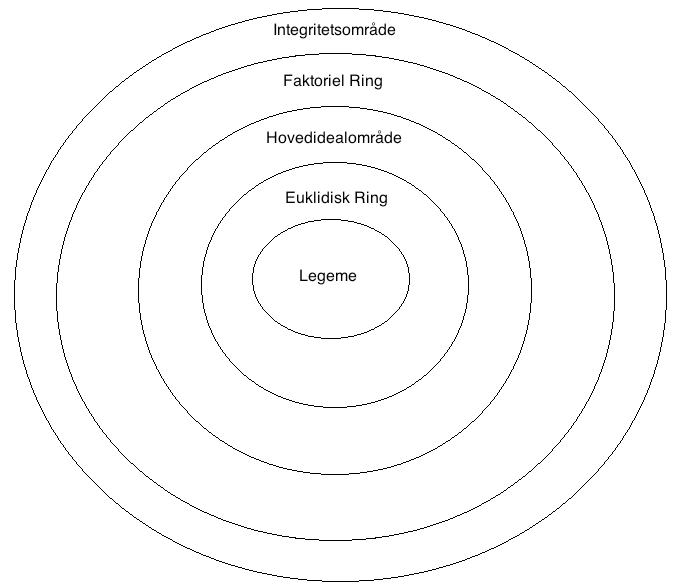
\includegraphics[width=0.8\textwidth]{img/ring_classes}












\newpage

\section{Polynomier (4)}
\subsection{Polynomiumsringe (4.1)}
\label{Polynomiumsringe (4.1)}
Lad $R$ være en \nameref{Ring} og $R[\N]$ mængden af afbildninger
\begin{equation*}
  f: \N \rightarrow R
\end{equation*}
sådan at $f(n) = 0$ for $n \gg 0$, hvilket vil sige at der findes et tal $N$, så
$f(n)=0$ for alle $n>N$.

Givet $f,g \in R[\N]$ definerer vi deres sum 
\begin{align*}
  (f + g)(n) &= f(n) + g(n)\\
             &= (\aPoly) + (\bPoly)\\
             &= (a_0 + b_0) + (a_1 + b_1)x + \cdots + (a_n + b_n)x^n\\
             &= \sum_{i=0}^{n}a_i x^i + \sum_{i=0}^{n}b_i x^i\\ 
             &= \sum_{i=0}^{n}(a_i + b_i) x^i
\end{align*}
og deres produkt
\begin{align*}
  (fg)(n) &= f(n)g(n)\\
             &= (\aPoly)(\bPoly)\\
             &= (a_0 b_0) + (a_1 b_0 + a_0 b_1)x + (a_2 b_0 + a_1 b_1 + a_0
             b_2)x^2 + \cdots\\
             &= \sum_{i=0}^{n}a_i x^i \sum_{j=0}^{n}b_i x^i\\
             &= \sum_{k=0}^{2n} \sum_{i+j = k}(a_i b_j)x^k
\end{align*}

Vi lader $X^i \in R[\N]$ være afbildningen
\begin{equation*}
  X^i(n) =  
  \left\{ 
  \begin{array}{l l}
    1 & \quad \text{if $n = i$}\\
    0 & \quad \text{if $n \neq i$}\\
  \end{array} \right.
\end{equation*}

Vi lader nu elementerne i ringen $a \in R$ være givet ved afbildningen
\begin{equation*}
    a(n) =  
  \left\{ 
  \begin{array}{l l}
    a & \quad \text{if $n = 0$}\\
    0 & \quad \text{if $n > 0$}\\
  \end{array} \right.
\end{equation*}

Derved kan et element $f \in R[\N]$ skrives som
\begin{equation*}
  f = \aPolyX
\end{equation*}
hvor $a_i = f(i)$ og $f_i = 0$ hvis $i > n$.

\subsubsection{Polynomiumsring}
\label{Polynomiumsring}
Vi definerer polynomiumsringen $R[X]$ i en variabel over \nameref{Ring}en $R$,
som $R[\N]$. $X = X^1 \in R[\N]$. Et polynomium $f \in R[X]$ kan skrives
\begin{equation*}
  \aPolyX
\end{equation*}
\begin{enumerate}[(i)]
  \item Et \textit{led} er et polynomium på formen $aX^m$, hvor $a \in
  R\setminus \myset{0}$.
  \item $a_0,\ldots,a_n \in R$ kaldes f's koefficienter.
  \item Hvis $a_n \neq 0$ er $deg(f) = n$ og $a_n$ er den ledende koefficient.
  \item $deg(f)$ kaldes graden af $f$ og $a_{deg(f)}X^{deg(f)}$ er det ledende
  led.
  \item Et ikke-nul polynomium kaldes normeret hvis dets ledende koefficient er
  1.
\end{enumerate} 

\subsubsection{Bemærkning 4.1.3}
\label{Bemaerkning 4.1.3}
To polynomier $f = \aPolyX$ og $g = \bPolyXm$ i $R[X]$ er ens $\iff a_0 =
b_0, a_1=b_1,\ldots$. Dette giver også mening når vi ser polynomier som
afbildninger $f: \N \rightarrow R$, hvor to afbildninger er ens $\iff$ de
afbilder til samme værdi for alle $n \in N$.

\subsection{Division af Polynomier (4.2)}
\label{Division af Polynomier}
\subsubsection{Prop. 4.2.2}
\label{Prop. 4.2.2}
Lad $f, g \in R[X] \mysetminus{0}$. Hvis den ledende koefficient af $f$ eller
$g$ ikke er en \nameref{Nuldivisor} gælder
\begin{equation*}
  deg(fg) = deg(f) + deg(g)
\end{equation*}

\subsubsection{Prop. 4.2.3}
\label{Prop. 4.2.3}
Lad $R$ være et \nameref{Integritetsomraade}. Så er $R[X]^* = R^*$.

\subsubsection{Prop. 4.2.4}
\label{Prop. 4.2.4}
Lad $d \in R[X]$ være et ikke-nul polynomium. Antag at den ledende koefficient
af $d$ ikke er en \nameref{Nuldivisor} i $R$. Givet $f \in R[X]$, eksisterer der
polynomier $q,r \in R[X]$ sådan at
\begin{equation*}
  f = qd + r
\end{equation*}
hvor $r = 0$ eller at $d$'s ledende led ikke dividerer nogle af $r$'s led. Se
\nameref{Entydig rest}.

\subsubsection{Korollar 4.2.5}
\label{Korollar 4.2.5}
Lad $d \in R[X]$ være et ikke-nul polynomium. Antag at den ledende koefficient
af $d$ er invertibel (er en \nameref{Enhed}) i $R$. Givet $f \in R[X]$,
eksisterer der polynomier $q,r \in R[X]$ sådan at
\begin{equation*}
  f = qd + r
\end{equation*}
hvor $r = 0$ eller $deg(r) < deg(d)$.

\subsubsection{Def. 4.2.7}
\label{Def. 4.2.7}
Polynomiet $r$ i \nameref{Korollar 4.2.5} kaldes resten af $f$ divideret med
$d$.


\subsection{Polynomiumsrødder (4.3)}
\label{Polynomiumsroedder (4.3)}
Afbildningen
\begin{equation*}
  j: R \rightarrow R[X]
\end{equation*}
givet ved $j(r) = r + 0X + 0X^2 + \cdots$ er en \nameref{Injektiv}
\nameref{Ringhomomorfi}. Billedet $j(R) = R$ og derved ser vi $R$ som en
\nameref{Delring} af $R[X]$.

\subsubsection{Prop. 4.3.1}
\label{Prop. 4.3.1}
Lad $f = \aPolyX \in R[X]$ og $\alpha \in R$. Afbildningen
$\phi_\alpha: \R[X] \rightarrow R$ givet ved
\begin{equation*}
  \phi_\alpha(f) = a_0 + a_1 \alpha + \cdots + a_n \alpha^n 
\end{equation*}
er en \nameref{Ringhomomorfi}.

\textit{Vi holder altså et $\alpha$ fast og givet et vilkårligt polynomium kan
vi indsætte dette $\alpha$ i stedet for $X$ og få en \nameref{Ringhomomorfi}.}

\subsubsection{Rod}
\label{Rod}
Lad $f \in R[X]$ være et polynomium. Elementet $\alpha \in R$ siges at være en
rod i $f$ hvis $f(\alpha) = \phi_\alpha(f) = 0$.

Vi lader $V(f) = \myset{\alpha \in R \mid f(\alpha) = 0}$ være mængden af rødder
for $f \in R[X]$.

\subsubsection{Korollar 4.3.2}
\label{Korollar 4.3.2}
Lad $f \in R[X]$. Så er $\alpha \in R$ en \nameref{Rod} i $f \iff$ $X - \alpha
\mid f$.

\subsubsection{Multiplicitet af en rod}
\label{Multiplicitet af en rod}
Multipliciteten af en \nameref{Rod} $\alpha$ i et ikke-nul polynomium $f$ er den
største potens $n \in \N$ sådan at
\begin{equation*}
  (X - \alpha)^n \mid f
\end{equation*}
Multipliciteten af $\alpha$ i $f$ skrives $\nu_\alpha (f)$. Bemærk at
\begin{enumerate}[(i)]
  \item $\nu_\alpha (f) \leq deg(f)$.
  \item $f = (X - \alpha)^{\nu_\alpha(f)}h$, hvor $h(\alpha) \neq 0$.
\end{enumerate}

\subsubsection{Multipel rod}
\label{Multipel rod}
En multipel rod i $f$ er en \nameref{Rod} $\alpha \in R$ med $\nu_\alpha(f) >
1$.

\subsubsection{Lemma 4.3.4}
\label{Lemma 4.3.4}
Lad $R$ være et \nameref{Integritetsomraade} og $f,g \in R[X]$. Så gælder
\begin{equation*}
  V(fg) = V(f) \cup V(g)
\end{equation*}

\subsubsection{Sætning 4.3.5}
\label{Saetning 4.3.5}
Lad $R$ være et \nameref{Integritetsomraade} of $f \in R[X]\mysetminus{0}$. Hvis
$V(f) = \myset{\alpha_1, \ldots,\alpha_r}$ så
\begin{equation*}
  f = q(X - \alpha_1)^{\nu_{\alpha_1}(f)}\cdots(X -
  \alpha_r)^{\nu_{\alpha_r}(f)}
\end{equation*}
hvor $q \in R[X]$ og $V(q) = \emptyset$. Antallet af \nameref{Rod}der i $f$,
talt med multiplicitet, er bundet af graden af $f$, $deg(f)$.

\textit{NB. Gælder kun hvis $R$ er et \nameref{Integritetsomraade}, så ikke i
$\Z/n\Z$, hvor $n$ er sammensat f.eks.}.

\subsubsection{Differentiering af polynomier}
\label{Differentiering af polynomier}
Lad $R$ være en \nameref{Ring} og $f = a_0 + a_1 X + \cdots + a_{n-1} X^{n-1} +
a_n X^n \in R[X]$. Så siger vi
\begin{equation*}
  D(f) = a_1 + \cdots + a_{n-1}(n-1)X^{n-2} + a_n n X^{n-1}
\end{equation*}
er den afledede af $f$.

Når vi ser polynomier som afbildninger $f: \N \rightarrow R$, kan ovenstående
omformuleres til 
\begin{equation*}
  D(f)(n-1) = nf(n) \text{ for } n \geq 1
\end{equation*}

\subsubsection{Lemma 4.3.7}
\label{Lemma 4.3.7}
Lad $f,g \in R[X]$ og $\lambda \in R$. Så gælder
\begin{enumerate}[(i)]
  \item $D(f + g) = D(f) + D(g)$
  \item $D(\lambda f) = \lambda D(f)$
  \item $D(fg) = fD(g) + D(f)g$
\end{enumerate}

\subsubsection{Lemma 4.3.8}
\label{Lemma 4.3.8}
Lad $f,g \in R[X]$.
\begin{enumerate}[(i)]
  \item Hvis $f^2 \mid g \Rightarrow f \mid D(g)$
  \item Et element $\alpha \in R$ er en \nameref{Multipel rod} i $f \iff \alpha$
  er en \nameref{Rod} i $f$ og $D(f)$.
\end{enumerate}

\subsubsection{Bemærkning 4.3.9}
\label{Bemaerkning 4.3.9}
Hvis \nameref{Polynomiumsring}en $R[X]$ har en primisk karakteristik $p > 0$
(\nameref{Karakteristik af en ring}) findes der mange ikke-konstante polynomier
$f \in R[X]$, hvor $D(f) = 0$.

F.eks. $X^p \in $ \nameref{F_p}$[X]$. Her er
\begin{equation*}
  D(X^p) = pX^{p-1} = 0
\end{equation*}
da $X^{p-1} \mycong {1}{p}$ ifølge \nameref{Fermats lille saetning}.

Generelt gælder $D(X^n) = 0 \iff p \mid n$ når $X^n \in \F_p [X]$.

\subsection{Cyklotomiske polynomier (4.4)}
\label{Cyklotomiske polynomier (4.4)}
\subsubsection{Enhedsrod}
\label{Enhedsrod}
Et komplekst tal $\xi$ siges at være en enhedsrod af $n$-te grad for et $n \in
\N$ hvis $\xi^n = 1$.

Skriver vi enhedsroden $\xi$ i polære koordinater $re^{i\theta} = r(\cos\theta
+ i \sin \theta)$ følger det at $r = 1$ og $\theta = k2\pi i/n$ for $k =
0,\ldots,n-1$, hvis $\xi$ er af $n$-te grad.

\subsubsection{Lemma 4.4.1}
\label{Lemma 4.4.1}
Et komplekst tal $\zeta$ er en \nameref{Primitiv enhedsrod} af $n$-te grad
$\iff$
\begin{equation*}
  \zeta = e^{k2\pi i/n}
\end{equation*}
hvor $1 \leq k \leq n$ og $gcd(k,n) = 1$. Husk fra \nameref{Enhedsrod} at
$\theta = k2\pi i/n$.

Hvis $\zeta$ er en primitiv enhedsrod af $n$-te grad og $\zeta^m \Rightarrow n
\mid m$.

\subsubsection{Bemærkning}
\label{Bemaerkning}
Mængden af enhedsrødder af $n$-te grad er en \nameref{Undergruppe} af $\C^*$.
Denne undergruppe er isomorf til den \nameref{Cyklisk gruppe} $\Z/n\Z$.

\subsubsection{Cyklotomisk polynomium}
\label{Cyklotomisk polynomium}
Def. 4.4.2: Lad $n \in \N$ hvor $n \geq 1$. Det $n$-te cyklotomiske polynomium
er defineret som polynomiet
\begin{equation*}
  \Phi_n(X) = \prod_{1 \leq k \leq n,\text{ } gcd(k,n1)=1} (X - e^{k2\pi i/n})
\end{equation*}
i $\C[X]$.

Et cyklotomisk polynomium er et polynomium hvis rødder er alle
\nameref{Primitiv enhedsrod}er af $n$-te grad. Det ses at det opfylder
\nameref{Lemma 4.4.1}.

Bemærk at $deg(\Phi_n) = \phi(n)$

Koefficienterne af $\Phi_n$ er altid $= \pm 1$ hvis $n$ er et produkt af two
forskellige \nameref{Primtal}. Se side 156 for at se de 4 første cykoltomiske
polynomier.

\subsubsection{Prop. 4.4.3}
\label{Prop. 4.4.3}
Lad $n \geq 1$. Så gælder
\begin{enumerate}[(i)]
  \item $X^n - 1 = \prod_{d\mid n} \Phi_d(X)$
  \item Et \nameref{Cyklotomisk polynomium} har heltalskoefficienter
  \begin{equation*}
    \Phi_n(X) \in \Z[X]
  \end{equation*}
\end{enumerate}

Lad $R$ være en \nameref{Ring}. Den \nameref{Entydig ringhomomorfi fra Z}
$\kappa: \Z \rightarrow R$ giver en \nameref{Ringhomomorfi}.
\begin{equation*}
  \kappa': \Z[X] \rightarrow R[X]
\end{equation*}
På denne måde kan vi se et \nameref{Cyklotomisk polynomium} $\Phi_n (X) \in
\Z[X]$ som polynomiet $\kappa'(\Phi_n) \in R[X]$. Dette leder os tilbage til
identiteten
\begin{equation*}
  X^n - 1 = \prod_{d\mid n} \Phi_d(X)
\end{equation*}
i $R[X]$ ved at anvende $\kappa'$ på den tilsvarende identitet i $\Z[X]$.

\subsection{Primitive rødder (4.5)}
\label{Primitive roedder (4.5)}

\subsubsection{Primitiv enhedsrod}
\label{Primitiv enhedsrod}
Def. 4.5.1: Lad $R$ være en \nameref{Ring} og $n \in \N\mysetminus{0}$. Et
element $\alpha \in R$ siges at være en primitiv \nameref{Enhedsrod} af $n$-te grad i $R$ hvis
$\alpha^n = 1$ og
\begin{equation*}
  a,a^2,..,a^{n-1} \neq 1
\end{equation*}
hvor $n \geq 1$.

\subsubsection{Lemma 4.5.2}
\label{Lemma 4.5.2}
Lad $\alpha \in R$, hvor $R$ er et \nameref{Integritetsomraade}. Hvis
$\Phi_n(\alpha) = 0$ og $\alpha$ ikke er en \nameref{Multipel rod} i $X^n - 1
\in R[X] \Rightarrow \alpha$ er en \nameref{Primitiv enhedsrod} af $n$-te grad i
$R$.

\subsubsection{Sætning 4.5.3 (Gauss)}
\label{Saetning 4.5.3 (Gauss)}
Lad $\F$ være et \nameref{Legeme} og $G \subseteq \F^*$ en endelig
\nameref{Undergruppe} af \nameref{Enhed}erne i $\F$. Så er $G$ en
\nameref{Cyklisk gruppe}.

Denne sætning viser at \nameref{F_p}$^*$ er en cyklisk gruppe, hvor $p$ er
et \nameref{Primtal}.

Et heltal $a$, sådan at $[a]$ frembringer $\F_p^*$, kaldes en primitiv rod
modulo $p$. En primitiv rod $a$ modulo $p$ tilfredsstiller
\begin{equation*}
  \F_p^* = \myset{[1], [a],[a^2],\ldots,[a^{p-2}]}
\end{equation*}
Se side 159 for mere om primitive rødder modulo $p$.

\subsection{Idealer i polynomiumsringe (4.6)}
\label{Idealer i polynomiumsringe (4.6)}

\subsubsection{Prop. 4.6.1}
\label{Prop. 4.6.1}
Polynomiumsringen $\F[X]$, hvor $\F$ er et \nameref{Legeme} er en
\nameref{Euklidisk ring}, et \nameref{Hovedidealomraade} og et
\nameref{Faktoriel ring}.

\subsubsection{Prop. 4.6.3}
\label{Prop. 4.6.3}
Lad $ f \in \F[X]$. Så gælder
\begin{enumerate}[(i)]
  \item \nameref{Ideal}et $\langle f \rangle$ er et \nameref{Maksimalt ideal}
  $\iff f$ er et \nameref{Irreducibelt element}. I dette tilfælde er
  \nameref{Kvotientring}en
  \begin{equation*}
    \F[X]/\langle f \rangle
  \end{equation*}
  et \nameref{Legeme}.
  
  \item Hvis $f \neq 0$ så er $f$ en \nameref{Enhed} $\iff deg(f) = 0$.
  \item Hvis $deg(f) = 1$ så er $f$ et \nameref{Irreducibelt
  element}.
  \item Hvis $f$ er irreducibelt og $deg(f) > 1$ har $f$ ingen
  \nameref{Rod}der.
  \item Hvis $deg(f) = 2$ \textit{eller} $deg(f) = 3$ så er $f$ irreducibelt
  $\iff f$ ingen rødder har.
\end{enumerate}
Se s. 164-165 for yderligere småting omkring idealer.

\subsubsection{Prop. 4.6.7}
\label{Prop. 4.6.7}
Lad $R$ være en \nameref{Ring} og
\begin{equation*}
  f = \aPolyX \in R[X]
\end{equation*}
et normeret (ledende koeff = 1) polynomium med $deg(f) = n > 0$. 

\begin{enumerate}[(i)]
  \item Så er $R \cap \langle f \rangle = \langle 0 \rangle$.
  \item Elementerne $[g] = g + \langle f \rangle$ i \nameref{Kvotientring}en
$R[X]/\langle f \rangle$ kan entydigt udtrykkes som polynomier af grad $ < n$
\begin{equation*}
  b_0 + b_1 \alpha + \cdots + b_{n-1}\alpha^{n-1}
\end{equation*}
hvor $b_0,\ldots,b_{n-1} \in R$ og $\alpha = [X]$.
  \item I $R[X]/\langle f \rangle$ har vi identiteten
\begin{equation*}
  \alpha^n = - a_0 -a_1 \alpha - \cdots - a_{n-1}\alpha^{n-1}
\end{equation*}
\end{enumerate}
Bemærk at $R$ er en naturlig \nameref{Delring} af $R[X]/\langle f \rangle$. Den
naturlige
\nameref{Ringhomomorfi}
\begin{equation*}
  \phi: R \rightarrow R[X]/\langle f \rangle
\end{equation*}
givet ved $\phi(r) = [r]$ er \nameref{Injektiv}.

\subsubsection{Bemærkning 4.6.8}
\label{Bemaerkning 4.6.8}
Hvis $\F$ er et \nameref{Legeme} og $f\in \F[X]$ er et \nameref{Irreducibelt
element} så er $\langle f \rangle$ et \nameref{Hovedideal} og derved bliver
$\F[X]/\langle f \rangle$ et udvidelseslegeme $E$ til $\F$.

Nu viser det sig at $\alpha = [X] \in E$ og er en \nameref{Rod} til $f \in
\F[X] \subseteq E[X]$, da $f(\alpha) = 0$ fra \nameref{Prop. 4.6.7}.

\subsection{Endelige legemer (4.8)}
\label{Endelige legemer (4.8)}
\subsubsection{Lemma 4.8.1}
\label{Lemma 4.8.1}
Lad $\F$ være et endeligt \nameref{Legeme}. Så er $|\F| = p^n$, hvor $p$ er et
\nameref{Primtal}, $n \geq 1$ og der eksisterer et \nameref{Irreducibelt
element} $f \in \F_{p}[X]$ af grad $n$, sådan at
\begin{equation*}
  \F \cong \F_p[X]/\langle f \rangle
\end{equation*}

\subsubsection{Sætning 4.8.2}
\label{Saetning 4.8.2}
Der eksisterer et entydigt endeligt \nameref{Legeme} med $p^n$ elementer, hvor
$p$ er et primtal og $n \geq 1$. Der gælder yderligere
\begin{enumerate}[(i)]
  \item Der eksisterer et \nameref{Irreducibelt element} i $\F_p [X]$ af grad
  $n$.
  \item Antag at $\F$ og $\F$' er endelige legemer med $p^n$ elementer. Så
  eksisterer der er Ringisomorfi (\nameref{Ringhomomorfi}) $\F \myisomto
  \F'$.
\end{enumerate}

\subsubsection{Lemma 4.8.3}
\label{Lemma 4.8.3}
Lad $\tau, d, n \in \N$, hvor $\tau > 1$. Så $t^d - 1 \mid t^n -1 \iff d \mid
n$.

\subsubsection{Sætning 4.8.5}
\label{Saetning 4.8.5}
Der eksisterer et \nameref{Irreducibelt element} i $\F_p [X]$ af grad $n \geq
1$. Hvis $f$ er irreducibelt og $f \mid \Phi_{p^n - 1}$ i $\F_p [X]$ så er
$deg(f) = n$.
\newpage

\section{Gröbner baser (5)}
\subsection{Polynomier i flere variable (5.1)}
\label{Polynomier i flere variable (5.1)}
Vi husker hvordan vi definerede en \nameref{Polynomiumsring} i en variabel. Vi
udvider nu dette til en polynomiumsring i flere variable $R[\myto{X_1}{X_n}]$
som
\begin{equation*}
  R[\myto{X_1}{X_n}] = R[\N^n] = 
  \myset{f : \N^n \to R \mid f(v) = 0, \myabs{v} \gg 0}
\end{equation*}
hvor $v = (\myto{v_1}{v_n}) \in \N^n$ og $\myabs{v} = v_1 + \cdots + v_n$.

Et polynomium $f \in R[\myto{X_1}{X_n}]$ er altså det samme som en afbildning
\begin{equation*}
  f: \N^n \to R
\end{equation*}
der er ikke-nul for kun endeligt mange $v$.

Vi lader $X^v \in R[\N^n]$ være afbildningen
\begin{equation*}
  X^v(w) =  
  \left\{ 
  \begin{array}{l l}
    1 & \quad \text{if $v = w$}\\
    0 & \quad \text{if $v \neq w$}\\
  \end{array} \right.
\end{equation*}

Med denne notation kan vi nu skrive polynomier i flere variable, $f \in
R[\N^n]$, som en endelig sum
\begin{equation*}
  f = \sum_{v \in N^n} a_v X^v
\end{equation*}
hvor $a_v \in R$.

Vi definerer addition af to polynomier $f, g \in R[\N^n]$ på følgende vis
\begin{equation*}
  f + g = (f + g)(v) = f(v) + g(v)
\end{equation*}

og multiplikation $fg$ som den endelige sum
\begin{equation*}
  (fg)(v) = \sum_{v_1 + v_2 = v} f(v_1) g(v_2)
\end{equation*}
hvor $v_1, v_2 \in \N^n$.

Bemærk at
\begin{enumerate}[(i)]
  \item $0 \in R$ er det neutrale element for $+$.
  \item Afbildningen $X^{(0,0,\ldots,0)}$ der afbilder 0-vektoren i $\N^n$ til
  $1 \in R$ og alt andet til $0 \in R$ til at være det neutrale element for
  $\cdot$.
\end{enumerate}

Ved notationen $R[\myto{X_1}{X_n}]$ for $R[\N^n]$ menes
\begin{enumerate}[(i)]
  \item $X_1 = X^{(1,0,\ldots,0)}$
  \item $X_2 = X^{(0,1,\ldots,0)}$
  \item $X_n = X^{(0,0,\ldots,1)}$
\end{enumerate}

Et \textit{led} er et polynomium $rX^v \in R[\N^n]$, hvor $r \in
R\mysetminus{0}$ kaldes \textit{koefficienten}.

Som eksempel kan vi skrive polynomiet $f$ op på to ens måder, en formel og en
konkret. De er ækvivalente
\begin{align*}
  f &= 2X^{(0,0,0)} + 2X^{(1,0,3)} + X^{(2,1,0)} - X^{(0,1,1)} + 3X^{(1,1,1)}
  \in \Z[\N^3]\\
    &= 2 + 2TZ^3 + T^2 Y - YZ + 3TYZ \in \Z[T,Y,Z] 
\end{align*}
hvor $T = X^{(1,0,0)}, Y = X^{(0,1,0)}$ og $Z = X^{(0,0,1)}$. Det formelle
polynomium er nu udtrykt ved de 3 variable $T,Y,Z$.



\subsubsection{Termordning}
\label{Termordning}
Def. 5.1.2: Mængden $\N^n$, bestående af $n$-tupler af naturlige tal, har en
komponentvis addition $+$ med nul-vektoren $0 = (0,\ldots,0)$. En
\nameref{Partiel ordning} $\leq$ på $\N^n$ kaldes en termordning hvis
\begin{enumerate}[(i)]
  \item $\leq$ er en \nameref{Total ordning}.
  \item $0 \leq v$
  \item $v_1 \leq v_2 \Rightarrow v_1 + v \leq v_2 + v$
\end{enumerate}
$\forall v, v_1, v_2 \in N^n$.

\subsubsection{Leksikografisk ordning}
\label{Leksikografisk ordning}
Vi definerer den leksikografiske ordning $\leq_{lex}$ på $\N^n$ ved
\begin{equation*}
  (v_1,\ldots,v_n) \leq_{lex} (w_1,\ldots,w_n)
\end{equation*}
hvis en af følgende gælder
\begin{align*}
  &(v_1 < w_1) \quad \text{eller}\\
  &(v_1 = w_1) \text{ og } (v_2 < w_2) \quad \text{eller}\\
  &(v_1 = w_1) \text{ og } (v_2 = w_2) \text{ og } (v_3 < w_3) \quad \text{etc}
\end{align*}
Dette vil sige normal alfabetisk ordning. F.eks. $(1,1,3) \leq_{lex} (1,2,3)$
da $1 < 2$ og $(4,5,1) \leq_{lex} (4,5,3)$ da $1 < 3$. Den leksikografiske
ordning er en \nameref{Termordning}.

\subsubsection{Graderet leksikografisk ordning}
\label{Graderet leksikografisk ordning}
Lad $\myabs{v} = v_1 + \cdots + v_n$, hvor $v = (v_1,\ldots,v_n) \in \N^n$. Vi
definerer nu den graderede leksikografiske ordning ved
\begin{equation*}
  (v_1,\ldots,v_n) \leq_{grlex} (w_1,\ldots,w_n)
\end{equation*}
hvis
\begin{align*}
  &\myabs{v} < \myabs{w} \quad \text{eller}\\
  &\myabs{v} = \myabs{w} \text{ og } v \leq_{lex} w
\end{align*}
F.eks. $(2,1,1) \leq_{grlex} (1,2,3)$, da $(2 + 1 + 1 < 1 + 2 + 3)$, selvom\\
$(2,1,1) \geq_{lex} (1,2,3)$. Den graderede leksikografiske ordning er en
\nameref{Termordning}.

\subsubsection{Lemma 5.1.5 (Dickson)}
\label{Lemma 5.1.5 (Dickson)}
Lad $S$ være en delmængde af $\N^n$. Så er der en endelig mængde af vektorer
$v_1,\ldots,v_r \in S$ sådan at
\begin{equation*}
  S \subseteq (v_1 + \N^n) \cup \cdots \cup (v_r + \N^n)
\end{equation*}
hvor $v_i + \N^n = \myset{v_i + w \mid w \in \N^n}$ for en vektor $v_i \in
\N^n$.

\subsubsection{Korollar 5.1.7}
\label{Korollar 5.1.7}
En \nameref{Termordning} $\leq$ på $\N^n$ er en \nameref{Velordning}.

\subsection{Initialterm (5.2)}
\label{Initialterm (5.2)}
\subsubsection{Initialterm}
\label{Initialterm}
Def. 5.2.1: Lad
\begin{equation*}
  f = \sum_{v \in \N^n} a_v X^v
\end{equation*}
være et ikke-nul polynomium i $R[\N^n]$ og $\leq$ er \nameref{Termordning} på
$\N^n$.

Initialtermet af $f$ mht. $\leq$ er defineret som
\begin{equation*}
  in_{\leq}(f) = a_w X^w
\end{equation*}
hvor $w = max_{\leq}\myset{v \in \N^n \mid a_v \neq 0}$.

F.eks. Lad
\begin{equation*}
  f = X^2 + XY + Y + Y^3 + X^5 \in \Z[X,Y]
\end{equation*}
hvor $X = X^{(1,0)}$ og $Y = X^{(0,1)}$ i $\Z[\N^n]$. Derved er
\begin{equation*}
  f = X^{(2,0)} + X^{(1,1)} + X^{(0,1)} + X^{(0,3)} + X^{(5,0)} \in \Z[\N^2]
\end{equation*}
Lader vi nu $\leq = \leq_{lex}$ får vi
\begin{equation*}
  (5,0) \geq (2,0) \geq (1,1) \geq (0,3) \geq (0,1)
\end{equation*}
Efter denne orden skulle man skrive $f = X^5 + X^2 + XY + Y^3 + Y$. Derved er
\begin{equation*}
  in_{\leq}(f) = X^5
\end{equation*}

\subsubsection{Bemærkning 5.2.3}
\label{Bemaerkning 5.2.3}
Lad $R$ være et \nameref{Integritetsomraade} og $f,g \in R[\myto{X_1}{X_n}]$.
Så gælder
\begin{equation*}
  in_{\leq}(fg) = in_{\leq}(f)in_{\leq}(g)
\end{equation*}
Dette er en analogt med \nameref{Prop. 4.2.2}, for polynomier i en variabel.

\subsection{Divisionsalgoritmen (5.3)}
\label{Divisionsalgoritmen (5.3)}
\subsubsection{Prop. 5.3.1}
\label{Prop. 5.3.1}
Prop. 5.3.1: Hold en \nameref{Termordning} $\leq$ på $\N^n$ fast. Lad $f \in
R[\myto{X_1}{X_n}] \mysetminus{0}$ og antag at $\myto{f_1}{f_m} \in
R[\myto{X_1}{X_n}]$ er en sekvens af ikke-nul polynomier. Så eksisterer der
$a_1,\ldots,a_m, r \in R[\myto{X_1}{X_n}]$ sådan at
\begin{equation*}
  f = a_1 f_1 + \cdots + a_m f_m + r
\end{equation*}
hvor $r = 0$ eller ingen af leddene i $r$ er delelig med
$in_{\leq}(f_1),\ldots,in_{\leq}(f_n)$. Desuden er $in_{\leq}(a_i f_i) \leq
in_{\leq}(f)$ hvis $f_i \neq 0$. Se \nameref{Prop. 4.2.4} for algoritmen i en
variabel.

\subsubsection{Def. 5.3.2}
\label{Def. 5.3.2}
Antag $f \in R[\myto{X_1}{X_n}]$ og lad $F = (f_1,\ldots,f_m)$ være en sekvens
af ikke-nul polynomier i $R[\myto{X_1}{X_n}]$. Vi lader $f^F$ beskrive resten
$r$ af $f$ efter division med $F$ vha. \nameref{Prop. 5.3.1}.

\subsection{Gröbnerbaser (5.4)}
\label{Gröbnerbaser (5.4)}

\subsubsection{Gröbnerbasis}
\label{Gröbnerbasis}
Lad $R$ være et \nameref{Legeme}.

En mængde af ikke-nul polynomier
\begin{equation*}
  F = (f_1,\ldots,f_m) \subseteq R[X_1,\ldots,X_n]
\end{equation*} 
kaldes en Gröbnerbasis for et \nameref{Ideal} i $R[X_1,\ldots,X_n]$ mht. en
\nameref{Termordning} $\leq$ hvis 
\begin{enumerate}[(i)]
  \item $F \subseteq I$
  \item For alle $f \in I \setminus{0}$,
  \begin{equation*}
    in{\leq}(f_i) \mid in_{\leq}(f)
  \end{equation*}
  for et $i = 1,\ldots,m$.
\end{enumerate}
Mængden $F$ kaldes en Gröbnerbasis mht en termordning $\leq$ hvis den er en
Gröbnerbasis for idealet \nameref{f_1..f_m} mht. $\leq$.

\subsubsection{Prop. 5.4.2}
\label{Prop. 5.4.2}
Lad $R$ være et \nameref{Legeme}. Lad $G = (f_1, \ldots, f_m)$ være en
\nameref{Gröbnerbasis} mht en \nameref{Termordning} $\leq$. For et polynomium
$f \in R[X_1,\ldots,X_n]$ har vi
\begin{equation*}
  f \in I \iff f^G = 0
\end{equation*}
hvor $I =$ \nameref{f_1..f_m}. Se \nameref{Def. 5.3.2} for $f^G$.

\subsubsection{Korollar 5.4.5}
\label{Korollar 5.4.5}
Lad $R$ være et \nameref{Legeme}. Lad $G = (f_1, \ldots, f_m) \subseteq
R[X_1,\ldots,X_n]$ være en \nameref{Gröbnerbasis} for \nameref{Ideal}et $I
\subseteq R$ mht en \nameref{Termordning}. Så er
\begin{equation*}
  I = \text{\nameref{f_1..f_m}}
\end{equation*}

\subsubsection{Prop. 5.4.6}
\label{Prop. 5.4.6}
Lad $R$ være et \nameref{Legeme}. Lad $G = (f_1, \ldots, f_m)$ være en
\nameref{Gröbnerbasis} i $R[X_1,\ldots,X_n]$ mht en \nameref{Termordning}
$\leq$. Så er den entydige rest $r$ i
\begin{equation*}
  f = a_1 f_1 + \cdots + a_m f_m + r
\end{equation*}
ligesom i \nameref{Prop. 5.3.1}, \textit{entydig} for alle $f \in R$.

Resten fra divisionsalgoritmen er uafhængig af rækkefølgen af elementerne $f_1,
\ldots, f_m \in G$.

\subsubsection{Sætning 5.4.7}
\label{Saetning 5.4.7}
Lad $k$ være et \nameref{Legeme}, $\leq$ en \nameref{Termordning} og $I
\subseteq k[X_1,\ldots,X_n]$ et \nameref{Ideal}. Så har $I$ en
\nameref{Gröbnerbasis} mht $\leq$.

\subsubsection{Korollar 5.4.8}
\label{Korollar 5.4.8}
Lad $R$ være et \nameref{Legeme}. Lad $I$ være et arbitrært \nameref{Ideal} i
$R[X_1,\ldots,X_n]$. Så er der endeligt mange polynomier $f_1,\ldots,f_m \in I$
sådan at ethvert polynomium $f \in I$ kan skrives
\begin{equation*}
  f = a_1 f_1 + \cdots + a_m f_m
\end{equation*}
for passende $a_1,\ldots,a_m \in R[X_1,\ldots,X_n]$, hvilket vil sige $I =$
\nameref{f_1..f_m}.

\subsubsection{S-polynomiet}
\label{S-polynomiet}
Def. 5.6.5: S-polynomiet af to ikke-nul polynomier $f$ og $g$ mht en
\nameref{Termordning} $\leq$ er defineret som
\begin{equation*}
  S(f,g) = \frac{X^w}{in_{\leq}(f)}f - \frac{X^w}{in_{\leq}(g)}g
\end{equation*}
hvor $X^w$ er $lcm(in_{\leq}(f), in_{\leq}(g))$.

\subsection{Newton Genvisit (5.5)}
\label{Newton Genvisit (5.5)}
\subsubsection{Sætning 5.5.1}
\label{Saetning 5.5.1}
Lad $f,f_1,\ldots,f_r \in k[X_1,\ldots,X_n]$. Lad $I$ være idealet
\begin{equation*}
  I = \langle T_1 - f_1,\ldots, T_r - f_r \rangle
\end{equation*}
i \nameref{Polynomiumsring}en $A = k[X_1,\ldots,X_n,T_1,\ldots,T_r]$ og $\leq$
være den \nameref{Leksikografisk ordning} givet ved
\begin{equation*}
  T_r \leq \cdots \leq X_n \leq \cdots \leq X_1
\end{equation*}
Lad $G$ være en \nameref{Gröbnerbasis} for $I$ mht $\leq$.

Så kan $f$ skrives som et polynomium i $f_1,\ldots,f_r \iff$
\begin{equation*}
  f^G \in k[T_1,\ldots,T_r]
\end{equation*}
I dette tilfælde er $f = f^G(f_1,\ldots,f_r)$.

\subsection{Buchbergers S-kriterie (5.6)}
\label{Buchbergers S-kriterie (5.6)}
\subsubsection{Korollar 5.6.9}
\label{Korollar 5.6.9}
En sekvens $F = (f_1, \ldots, f_m)$ af polynomier er en \nameref{Gröbnerbasis}
$\iff S(f_i, f_j)^F = 0$ for $1 \leq i \leq j \leq m$. Se \nameref{Def. 5.3.2}
for $S(f_i, f_j)^F$.

\subsection{Buchbergers algoritme (5.7)}
\label{Buchbergers algoritme (5.7)}
\subsubsection{Sætning 5.7.2}
\label{Saetning 5.7.2}
Buchberger's algoritme terminerer og outputtet er en \nameref{Gröbnerbasis}.

\subsection{Den reducerede Gröbnerbasis (5.8)}
\label{Den reducerede Gröbnerbasis (5.8)}
\subsubsection{Minimal Gröbnerbasis}
\label{Minimal Gröbnerbasis}
Def 5.8.1: En minimal gröbnerbasis $(f_1,\ldots,f_m)$ er en
\nameref{Gröbnerbasis} sådan at \begin{enumerate}[(i)]
  \item $in_{\leq}(f_j) \nmid in_{\leq}(f_i)$ for $i \neq j$.
  \item Koefficienten af $in_{\leq}(f_i)$ er 1.  
\end{enumerate}

\subsubsection{Reduceret Gröbnerbasis}
\label{Reduceret Gröbnerbasis}
Def 5.8.2: En reduceret gröbnerbasis $(f_1,\ldots,f_m)$ er en \nameref{Minimal
Gröbnerbasis} hvis $in_{\leq}(f_j) \nmid$ noget led i $f_i$ for $i \neq j$.

\subsubsection{Sætning 5.8.3}
\label{Saetning 5.8.3}
Lad $R$ være et \nameref{Legeme}. Ethvert ideal $I \subseteq R[X_1,\ldots,X_n]$
har en entydig \nameref{Reduceret Gröbnerbasis}.

\subsection{Løsning af ligningssystemer vha Gröbnerbaser (5.9)}
\label{Loesning af ligningssystemer vha Grobnerbaser (5.9)}
\subsubsection{Sætning 5.9.1}
\label{Saetning 5.9.1}
Lad $R$ være et \nameref{Legeme} og $G = (f_1,\ldots,f_m)$ være en
\nameref{Gröbnerbasis} for et \nameref{Ideal} $I \subseteq R[X_1,\ldots,X_n]$
mht den \nameref{Leksikografisk ordning} $\geq$ givet ved $X_n \geq X_{n-1}
\geq \cdots \geq X_1$.

Så er $G \cap R[X_1,\ldots,X_i]$ en gröbnerbasis for idealet $I \cap
R[X_1,\ldots,X_i]$ i $R[X_1,\ldots,X_i]$.


\newpage

\section{Appendix (6)}
\label{Appendix (6)}
\subsection{Talteori (1)}
\subsubsection{Induktionsprincippet}
At mængden $\N$ har en \nameref{Velordning} vil sige at det har et første
element, hvilket vil sige $\exists s : s \leq x$ for alle $x \in \N$. Dette er
ækvivalent til matematisk induktion der siger:

Lad $P(n)$ være et udsagn hvor der for alle $n \geq 1$ gælder
\begin{enumerate}[(i)]
  \item $P(1)$ er sand.
  \item $P(n)$ er sand $\Rightarrow$ at $P(n + 1)$ er sand.
\end{enumerate}
så kan vi konkludere at $P(n)$ er sand for alle $n \geq 1$.

\subsubsection{Reference (1.1)}
Der gælder $1 + 2 + \cdots + n = \frac{n(n+1)}{2}$

\subsubsection{Grupper (2)}
\label{Grupper (2)}
\subsubsection{Veldefineret}
\label{Veldefineret}
En afbildning $f: X \to Y$ kaldes veldefineret hvis den afbilder alle elementer
i domænet $X$ til et element i codomænet $Y$.

\textit{Uanset valget af repræsentanter for sideklasser så afbilder de til
samme element}.

\subsubsection{Injektiv}
\label{Injektiv}
En afbildning $f: X \to Y$ kaldes injektiv hvis der gælder
\begin{equation*}
  \forall a, b \in X \Rightarrow \text{ hvis } f(a) = f(b), \text{ så er } a
  = b
\end{equation*}
\textit{Alle elementer i domænet X afbilder til et unikt element i Y
$\Rightarrow \mid X\mid \leq \mid Y\mid$}.

\subsubsection{Surjektiv}
\label{Surjektiv}
En afbildning $f: X \to Y$ kaldes surjektiv hvis der gælder
\begin{equation*}
  \forall y \in Y \exists x \in X, \text{ hvor } f(x) = y
\end{equation*}
\textit{Alle elementer i codomænet Y bliver ramt af et element i X $\Rightarrow
\mid X \mid \geq \mid Y\mid$}.

\subsubsection{Bijektiv}
\label{Bijektiv}
En afbildning $f: X \to Y$ kaldes bijektiv hvis den er både
\begin{enumerate}[(i)]
  \item \nameref{Injektiv}. \textit{Alle elementer i codomænet Y bliver ramt af
  et element i X $\Rightarrow \mid X\mid \geq \mid Y\mid$}.  
  \item \nameref{Surjektiv}. \textit{Alle elementer i domænet X afbilder til et
  unikt element i Y $\Rightarrow \mid X\mid \leq \mid Y\mid$}.
\end{enumerate}
\textit{Enhver afbildning der har en invers er bijektiv}

\subsubsection{\textit{Ker(f)}}
\label{Ker(f)}
Lad $f: G \rightarrow K$ være en \nameref{Gruppehomomorfi}, så er:
\begin{equation*}
  Ker(f) = \myset{g \in G \mid f(g) = e}
\end{equation*}
\textit{Kernen af f er mængden af alle elementer i G, som f afbilder til det
neutrale element i K}.

\subsubsection{\textit{f(G)}}
Lad $f: G \rightarrow K$ være en \nameref{Gruppehomomorfi}, så er:
\label{f(G)}
\begin{equation*}
  f(G) = \{f(g) \mid g \in G\} \subseteq K
\end{equation*}
\textit{Billedet af f er alle de elementer i K som f afbilder til fra G}.

\begin{figure}
\begin{center}
  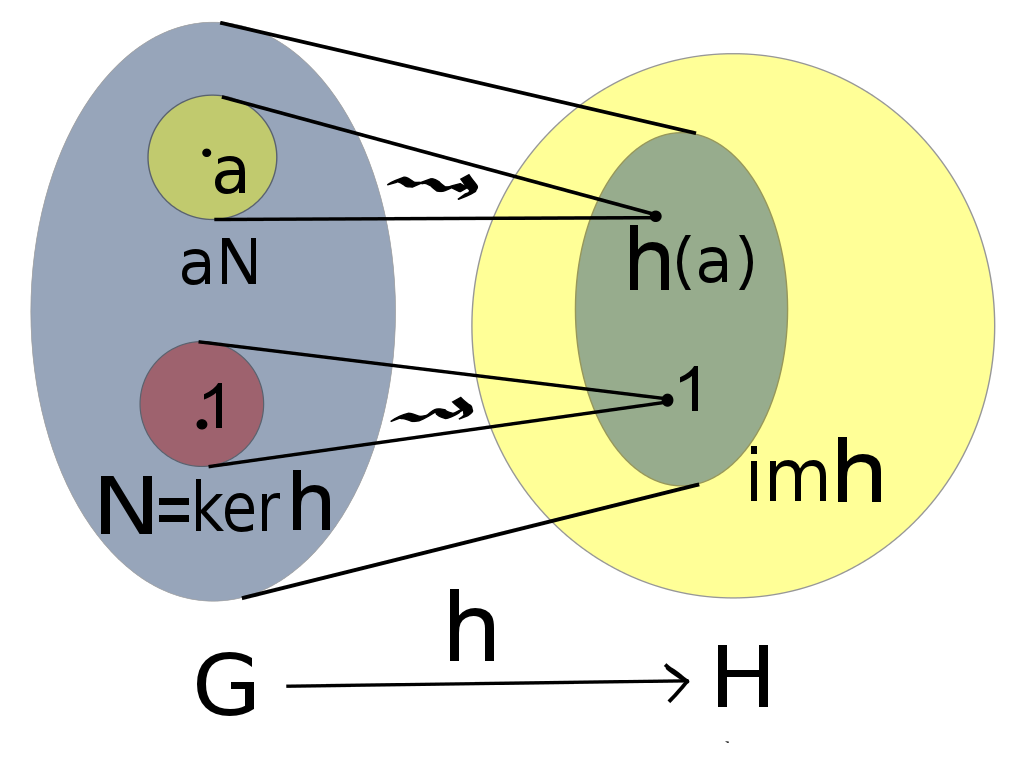
\includegraphics[width=0.8\textwidth]{img/group_homomorphism}
  \caption[labelInTOC]{
  Animation af en gruppehomomorfi $h: G \rightarrow H$. Den lille oval inde i
  $H$ er billedet af $H$. $N$ er kernen af $H$ og $aN$ er en sideklasse til
  $N$.}
  \label{figureLabel}
\end{center}
\end{figure}

\subsection{Gröbnerbaser (5)}
\label{Gröbnerbaser (5)}
\subsubsection{Relation}
\label{Relation}
Def. A.1.1: En relation $R$ på en mængde $S$ er en delmængde $R \subseteq S
\times S$. Vi skriver $xRy$ hvor vi mener $(x,y) \in R$.

\subsubsection{Ækvivalensrelation}
\label{Aekvivalensrelation}
Def. A.1.2: En \nameref{Relation} $R$ på en mængde $S$ er kaldes en
ækvivalensrelation hvis den er
\begin{enumerate}[(i)]
  \item Refleksiv: $xRx \quad \forall x \in S$.
  \item Symmetrisk: $xRy \Rightarrow yRx \quad \forall x,y \in S$.
  \item Transativ: $xRy \myand yRz \Rightarrow xRz \quad \forall x,y,z \in S$.
\end{enumerate}
som eksempel er kongruens modulo et ideal, $I$ en ækvivalensrelation
\begin{equation*}
  x \mycong{y}{I} \iff x - y \in I
\end{equation*}
Dette er det generelle tilfælde af relationen kongruens modulo et heltal i
$\Z$, hvilket også er en ækvivalensrelation.

\subsubsection{Partiel ordning}
\label{Partiel ordning}
Def. A.1.2: En \nameref{Relation} $R$ på en mængde $S$ er kaldes en partiel
ordning hvis den er
\begin{enumerate}[(i)]
  \item Refleksiv: $xRx \quad \forall x \in S$.
  \item Antisymmetrisk: $xRy \myand yRx \Rightarrow x = y \quad \forall x,y
  \in S$.
  \item Transativ: $xRy \myand yRz \Rightarrow xRz \quad \forall x,y,z \in S$.
\end{enumerate}
Som eksempel er $\leq$ en partiel ordning på $\Z$.

\subsubsection{Minimalt element}
\label{Minimalt element}
Et element $s \in S$ med en \nameref{Partiel ordning} $\leq$ siges at være et
minimalt element hvis
\begin{equation*}
  x \leq s \Rightarrow x = s
\end{equation*}
$\forall x \in S$.

\subsubsection{Første element}
\label{Foerste element}
Et element $t \in S$ med en \nameref{Partiel ordning} $\leq$ siges at være
et første element hvis
\begin{equation*}
  t \leq x
\end{equation*}
$\forall x \in S$. Fordi $\leq$ er antisymmetrisk må dette $t$ være unikt. Er
første element er et \nameref{Minimalt element}.

\subsubsection{Total ordning}
\label{Total ordning}
Def. A.3.4: En \nameref{Partiel ordning} $\leq$ på en mængde $S$ kaldes en total
ordning hvis
\begin{equation*}
  x \leq y \myor y \leq x \quad \forall x,y \in S
\end{equation*}

\subsubsection{Velordning}
\label{Velordning}
Def. A.3.5: En \nameref{Partiel ordning} $\leq$ på en mængde $S$ kaldes en
velordning hvis enhver ikke-tomt delmængde $M \subseteq S$ har et
\nameref{Foerste element}.

\subsection{$\langle f_1, \ldots, f_m \rangle$}
\label{f_1..f_m}
\begin{align*}
  &\langle f_1, \ldots, f_m \rangle =\\
  &\myset{a_1(X_1,\ldots,X_m)f_1 + \cdots + a_m(X_1,\ldots,X_m)f_m \mid
  a_1(X_1,\ldots,X_m), b_1(X_1,\ldots,X_m) \in R[X_1,\ldots,X_n]}
\end{align*}
hvilket vil sige alle ``lineære'' kombinationer af $f_1, \ldots, f_m$.
\newpage

\section{Eksamen (7)}
\subsection{Den kinesiske restklassesætning}
\label{Den kinesiske restklassesaetning}
Vi har et system.
\begin{align*}
  X &\mycong {a_1}{n_1}\\
  X &\mycong {a_2}{n_2}\\
  &\vdots\\
  X &\mycong {a_t}{n_t}
\end{align*}

Når vi har fundet vores $\lambda$'ere og $\mu$'ere er det blot at indsætte i
formlen
\begin{equation*}
  X = a_1 \mu_1 (N/n_1) + \cdots + a_t \mu_t (N/n_t)
\end{equation*}

\subsection{$\varphi(n)$}
Der gælder følgende om $\varphi(p^l)$, hvor $p$ er et primtal og $l \geq 1$.
\begin{align*}
  \varphi(p^k) = p^k -p^{k-1} =p^{k-1}(p-1) = p^k \left( 1 -
\frac{1}{p} \right)
\end{align*}
\textit{Proof: Since p is a primer number the only possible values of gcd(pk,m)
are 1, p, p2,\ldots, pk, and the only way for gcd(pk,m) to not equal 1 is for m
to be a multiple of p. The multiples of p that are less than or equal to pk are
p, 2p, 3p, \ldots, pk - 1p = pk, and there are pk - 1 of them. Therefore the
other $pk - pk - 1$ numbers are all relatively primt to pk.}

Yderemere gælder:
\begin{align*}
\varphi(n)
&= \varphi(p_1^{k_1}) \varphi(p_2^{k_2}) \cdots\varphi(p_r^{k_r})\\
&=  p_1^{k_1} \left(1- \frac{1}{p_1} \right) p_2^{k_2} \left(1- \frac{1}{p_2} \right) \cdots p_r^{k_r} \left(1- \frac{1}{p_r} \right)\\
&= p_1^{k_1} p_2^{k_2} \cdots p_r^{k_r} \left(1- \frac{1}{p_1} \right) \left(1- \frac{1}{p_2} \right) \cdots \left(1- \frac{1}{p_r} \right)\\
&=n \left(1- \frac{1}{p_1} \right)\left(1- \frac{1}{p_2} \right) \cdots\left(1- \frac{1}{p_r} \right).
\end{align*}
Eller kortere $\varphi(n) =n \prod_{p\mid n} \left(1-\frac{1}{p}\right)$,

Eksempel:
\begin{align*}
  \varphi(36)=\varphi\left(2^2
3^2\right)=36\left(1-\frac{1}{2}\right)\left(1-\frac{1}{3}\right)=36\cdot\frac{1}{2}\cdot\frac{2}{3}=12
\end{align*}

\subsection{Normafbildning}
Hvis $N(z_1 z_2) = N(z_1)N(z_2)$ og $N(1) = 1$ gælder
\begin{equation*}
  \text{Et element z $\in R$ er en \nameref{Enhed} $\iff N(z) = \pm 1$}
\end{equation*}
Bevis:
\begin{enumerate}[(i)]
  \item Hvis $z$ er en enhed så $\exists y$ sådan at $zy = 1$, derved $N(zy) =
  N(z)N(y)$ og derfor $N(z) = \pm 1$
  \item Hvis $N(z) = \pm 1$ så $z\varphi(z) = \pm 1$ og $z$ er en enhed.
\end{enumerate}
Dette er smart at udnytte når vi skal vise om et element er irreducibelt eller
ej.

\subsubsection{Vis at R ikke er et Hovedidealområde}
Nok at vise R ikke er en \nameref{Faktoriel ring}.
Generelt gælder at hvis et element har to forskellige faktoriseringer, og der
findes en faktor i den ene faktorisering der ikke går op i nogle af faktorerne
i den anden faktorisering, så er ringen \textit{ikke} en faktoriel ring.

\subsubsection{Antallet af frembringere i $L^*$}
Bevis 4.5.3 siger antallet af frembringere i $L^* = \varphi(|L^*|)$.

\subsubsection{Simple transpositioner}
Givet en cykel så start med at tæl inversionerne. Skriv den i 2-række form og
målet er nu at vi skal ende ud med identiteten. Vi skal bruge lige mange simple
transpositioner som der er inversioner.
\end{document}